\documentclass[conference]{IEEEtran}

\usepackage[T1]{fontenc}
\usepackage{amsmath,amssymb}
\usepackage{icomma}
\usepackage{booktabs}
\usepackage{graphicx}
\usepackage{cite}
\usepackage[hyphens]{url}
\def\UrlBreaks{\do\/\do\.\do\-}

% Automatically generated by paper/scripts/gen_numbers.py from analysis_root/out_addendum2/*.csv,
% analysis_root/out_addendum3/*.csv, raw run outputs (queries.npz, epochs.parquet, summary.json,
% failed_runs.json, RUN_ADD3.log), repo/results/pilot/, and constants from audit/M3_DESIGN_CHECK.md.
% Do not edit by hand.
\newcommand{\RNumAddThreeChargedDCForcedSumBFourNewTopic}{$16$}
\newcommand{\RNumAddThreeCompRows}{$32$}
\newcommand{\RNumAddThreeDCUnspentEpochBytes}{$24,448$}
\newcommand{\RNumAddThreeMOneRuns}{$10$}
\newcommand{\RNumAddThreeMThreeFailedAttempts}{$22$}
\newcommand{\RNumAddThreeMThreeRuns}{$30$}
\newcommand{\RNumAddThreePOneBound}{$-1.00$~pp}
\newcommand{\RNumAddThreePTwoBound}{$0.00$~pp}
\newcommand{\RNumAddThreeRNExtraEpochBytesVsChargedDC}{$21,504$}
\newcommand{\RNumAddThreeRNForcedSumBFourNewTopic}{$100$}
\newcommand{\RNumAddThreeRNMinusUnchargedDCBTwoNewTopicAbsMean}{$2.11$~pp}
\newcommand{\RNumAddThreeRepRuns}{$2$}
\newcommand{\RNumAddThreeTotalIntervals}{$64$}
\newcommand{\RNumAddThreeTotalRefreshesBFour}{$750$}
\newcommand{\RNumAddThreeTotalRuns}{$42$}
\newcommand{\RNumAddThreeXFourDCNewTopicCell}{$-0.63$ $[-0.89,$ $-0.38]$}
\newcommand{\RNumAddThreeXFourDCSteadyCell}{$+0.17$ $[-0.01,$ $+0.35]$}
\newcommand{\RNumAddThreeXFourESNewTopic}{$+0.38$~pp $[+0.01,$ $+0.74]$}
\newcommand{\RNumAddThreeXFourESNewTopicAbsMean}{$0.38$~pp}
\newcommand{\RNumAddThreeXFourESNewTopicBootLow}{$+0.01$~pp}
\newcommand{\RNumAddThreeXFourESNewTopicCell}{$+0.38$ $[+0.01,$ $+0.74]$}
\newcommand{\RNumAddThreeXFourESNewTopicEarlyMean}{$+0.68$~pp}
\newcommand{\RNumAddThreeXFourESNewTopicLateMean}{$-0.20$~pp}
\newcommand{\RNumAddThreeXFourESNewTopicTInt}{$[+0.13,$ $+0.64]$~pp}
\newcommand{\RNumAddThreeXFourESONewTopicCell}{$+0.43$ $[+0.07,$ $+0.79]$}
\newcommand{\RNumAddThreeXFourESOSteadyCell}{$-0.45$ $[-0.75,$ $-0.12]$}
\newcommand{\RNumAddThreeXFourESOverallNewTopic}{$-0.20$~pp $[-0.38,$ $+0.02]$}
\newcommand{\RNumAddThreeXFourESSteadyCell}{$-0.49$ $[-0.78,$ $-0.16]$}
\newcommand{\RNumAddThreeXFourPVNewTopicCell}{$-2.39$ $[-2.84,$ $-1.99]$}
\newcommand{\RNumAddThreeXFourPVSteadyCell}{$-1.54$ $[-1.96,$ $-1.12]$}
\newcommand{\RNumAddThreeXOneAllZeroGapBFourNewTopic}{$+5.42$~pp}
\newcommand{\RNumAddThreeXOneAllZeroQueriesBFourNewTopic}{$1,428$}
\newcommand{\RNumAddThreeXOneChoiceShareBFour}{$74\%$}
\newcommand{\RNumAddThreeXOneNonZeroGapBFourNewTopic}{$+1.86$~pp}
\newcommand{\RNumAddThreeXOneNonZeroQueriesBFourNewTopic}{$4,947$}
\newcommand{\RNumAddThreeXOnePosSeedsBFourBEight}{$10$}
\newcommand{\RNumAddThreeXOneRNBEightNewTopicCell}{$+1.76$ $[+1.04,$ $+2.59]$}
\newcommand{\RNumAddThreeXOneRNBEightSteadyCell}{$+0.19$ $[-0.29,$ $+0.64]$}
\newcommand{\RNumAddThreeXOneRNBFourNewTopic}{$+2.66$~pp $[+1.46,$ $+4.00]$}
\newcommand{\RNumAddThreeXOneRNBFourNewTopicAbsMean}{$2.66$~pp}
\newcommand{\RNumAddThreeXOneRNBFourNewTopicCell}{$+2.66$ $[+1.46,$ $+4.00]$}
\newcommand{\RNumAddThreeXOneRNBFourNewTopicTInt}{$[+0.91,$ $+4.57]$~pp}
\newcommand{\RNumAddThreeXOneRNBFourSteadyCell}{$+0.19$ $[-0.29,$ $+0.63]$}
\newcommand{\RNumAddThreeXOneRNBTwoNewTopicAbsMean}{$0.48$~pp}
\newcommand{\RNumAddThreeXOneRNBTwoNewTopicCell}{$+0.48$ $[-0.48,$ $+1.66]$}
\newcommand{\RNumAddThreeXOneRNBTwoSteadyCell}{$+0.30$ $[-0.29,$ $+0.88]$}
\newcommand{\RNumAddThreeXOneRNOverallBFourNewTopic}{$+0.42$~pp $[+0.11,$ $+0.69]$}
\newcommand{\RNumAddThreeXThreeDCBEightNewTopic}{$+0.16$~pp $[-0.10,$ $+0.41]$}
\newcommand{\RNumAddThreeXThreeDCBEightNewTopicCell}{$+0.16$ $[-0.10,$ $+0.41]$}
\newcommand{\RNumAddThreeXThreeDCBEightSteadyCell}{$+0.00$ $[-0.17,$ $+0.19]$}
\newcommand{\RNumAddThreeXThreeDCBFourNewTopicAbsMean}{$0.94$~pp}
\newcommand{\RNumAddThreeXThreeDCBFourNewTopicCell}{$-0.94$ $[-1.55,$ $-0.32]$}
\newcommand{\RNumAddThreeXThreeDCBFourSteadyCell}{$-0.20$ $[-0.71,$ $+0.30]$}
\newcommand{\RNumAddThreeXThreeDCBTwoNewTopicAbsMean}{$1.63$~pp}
\newcommand{\RNumAddThreeXThreeDCBTwoNewTopicCell}{$-1.63$ $[-2.90,$ $-0.48]$}
\newcommand{\RNumAddThreeXThreeDCBTwoSteadyCell}{$+0.33$ $[-0.39,$ $+1.08]$}
\newcommand{\RNumAddThreeXTwoESOBEightNewTopicCell}{$+1.63$ $[+0.27,$ $+2.95]$}
\newcommand{\RNumAddThreeXTwoESOBEightNewTopicNegSeed}{$42$}
\newcommand{\RNumAddThreeXTwoESOBEightNewTopicNegSeedGap}{$-0.17$~pp}
\newcommand{\RNumAddThreeXTwoESOBEightNewTopicTInt}{$[+0.10,$ $+3.17]$~pp}
\newcommand{\RNumAddThreeXTwoESOBEightSteadyCell}{$-4.28$ $[-5.17,$ $-3.42]$}
\newcommand{\RNumAddThreeXTwoESOBFourNewTopicCell}{$+2.92$ $[+1.39,$ $+4.26]$}
\newcommand{\RNumAddThreeXTwoESOBFourSteadyCell}{$-2.29$ $[-2.90,$ $-1.68]$}
\newcommand{\RNumAddThreeXTwoESOBTwoNewTopicCell}{$+1.12$ $[-0.39,$ $+2.62]$}
\newcommand{\RNumAddThreeXTwoESOBTwoSteadyCell}{$-0.87$ $[-1.41,$ $-0.36]$}
\newcommand{\RNumAddThreeXTwoESOOverallBEightNewTopic}{$-3.43$~pp $[-3.77,$ $-3.02]$}
\newcommand{\RNumAddThreeXTwoESOOverallBFourNewTopic}{$-0.79$~pp $[-1.26,$ $-0.25]$}
\newcommand{\RNumAddThreeXTwoPVBEightNewTopicCell}{$-3.42$ $[-5.15,$ $-1.75]$}
\newcommand{\RNumAddThreeXTwoPVBEightSteadyCell}{$-7.16$ $[-7.98,$ $-6.33]$}
\newcommand{\RNumAddThreeXTwoPVBFourNewTopicCell}{$+0.10$ $[-1.40,$ $+1.52]$}
\newcommand{\RNumAddThreeXTwoPVBFourSteadyCell}{$-3.87$ $[-4.72,$ $-3.11]$}
\newcommand{\RNumAddThreeXTwoPVBTwoNewTopic}{$-0.16$~pp $[-1.89,$ $+1.49]$}
\newcommand{\RNumAddThreeXTwoPVBTwoNewTopicCell}{$-0.16$ $[-1.89,$ $+1.49]$}
\newcommand{\RNumAddThreeXTwoPVBTwoNewTopicTInt}{$[-2.56,$ $+2.18]$~pp}
\newcommand{\RNumAddThreeXTwoPVBTwoSteadyCell}{$-1.58$ $[-2.11,$ $-1.06]$}
\newcommand{\RNumAddThreeXTwoPVOverallBTwoNewTopic}{$+0.62$~pp $[+0.35,$ $+0.90]$}
\newcommand{\RNumAddendumTwoMTwoDone}{$140/330$}
\newcommand{\RNumAlwaysFreshEpochBytes}{$786,432$}
\newcommand{\RNumBootNarrowerMax}{$27\%$}
\newcommand{\RNumBootNarrowerMin}{$19\%$}
\newcommand{\RNumBootSeed}{$42$}
\newcommand{\RNumBootWiderMThreeRNMinusQLNewTopic}{$51\%$}
\newcommand{\RNumBudgetBFourEpochBytes}{$98,304$}
\newcommand{\RNumCIPct}{$95\%$}
\newcommand{\RNumCentersPerSummary}{$16$}
\newcommand{\RNumChanceRecallMTwo}{$0.0625$}
\newcommand{\RNumCorpusTotalPassages}{$100,000$}
\newcommand{\RNumDCScoreEpochBytes}{$128$}
\newcommand{\RNumDataSeed}{$42$}
\newcommand{\RNumESLoadPctBEight}{$29.5\%$}
\newcommand{\RNumESLoadPctBFour}{$14.8\%$}
\newcommand{\RNumESLoadPctBTwo}{$7.2\%$}
\newcommand{\RNumESLoadPctQEightHundred}{$3.7\%$}
\newcommand{\RNumESLoadPctQFifty}{$59.0\%$}
\newcommand{\RNumESLoadPctQTwoHundred}{$14.8\%$}
\newcommand{\RNumESOQFiftyMaxSearches}{$50$}
\newcommand{\RNumEpochsPerCondition}{$250$}
\newcommand{\RNumExtraSearchesBFour}{$59$}
\newcommand{\RNumFiveSeeds}{$5$}
\newcommand{\RNumForcedShareDCNewTopicMOne}{$6.9\%$}
\newcommand{\RNumForcedShareDCSteadyMOne}{$0.0\%$}
\newcommand{\RNumForcedShareQLNewTopicMOne}{$27.3\%$}
\newcommand{\RNumForcedShareQLSteadyMOne}{$27.9\%$}
\newcommand{\RNumForcedShareRNNewTopicMOne}{$21.7\%$}
\newcommand{\RNumForcedShareRNNewTopicMOneQEightHundred}{$21.7\%$}
\newcommand{\RNumForcedShareRNNewTopicMOneQFifty}{$21.7\%$}
\newcommand{\RNumForcedShareRNNewTopicMThree}{$13.3\%$}
\newcommand{\RNumForcedShareRNNewTopicMThreeBEight}{$5.3\%$}
\newcommand{\RNumForcedShareRNNewTopicMThreeBTwo}{$0.0\%$}
\newcommand{\RNumForcedShareRNSteadyMOne}{$27.2\%$}
\newcommand{\RNumForcedShareRNSteadyMOneQEightHundred}{$27.2\%$}
\newcommand{\RNumForcedShareRNSteadyMOneQFifty}{$27.2\%$}
\newcommand{\RNumForcedShareRNSteadyMThree}{$17.2\%$}
\newcommand{\RNumForcedShareRNSteadyMThreeBEight}{$5.0\%$}
\newcommand{\RNumForcedShareRNSteadyMThreeBTwo}{$0.0\%$}
\newcommand{\RNumForcedShareSSNewTopicMOne}{$26.9\%$}
\newcommand{\RNumForcedShareSSSteadyMOne}{$28.0\%$}
\newcommand{\RNumFourRulesSummariesBTwo}{$2$}
\newcommand{\RNumGateMThreeNewTopic}{$+6.74$~pp $[+5.16,$ $+8.16]$}
\newcommand{\RNumGateMThreeNewTopicMinSeed}{$42$}
\newcommand{\RNumGateMThreeNewTopicMinSeedGap}{$+4.10$~pp}
\newcommand{\RNumGateMThreeNewTopicTInt}{$[+4.79,$ $+8.75]$~pp}
\newcommand{\RNumGateMThreeNewTopicUnweightedMean}{$+6.77$~pp}
\newcommand{\RNumGateMThreeOverallNewTopic}{$+1.73$~pp $[+1.12,$ $+2.33]$}
\newcommand{\RNumGateMThreeOverallSteady}{$-0.91$~pp $[-1.02,$ $-0.79]$}
\newcommand{\RNumGateMThreeSteady}{$+1.16$~pp $[+0.38,$ $+1.91]$}
\newcommand{\RNumGateMTwoNewTopic}{$+22.61$~pp $[+20.83,$ $+24.40]$}
\newcommand{\RNumGateMTwoOverallNewTopic}{$+9.87$~pp $[+8.87,$ $+10.77]$}
\newcommand{\RNumGateMTwoOverallSteady}{$-1.59$~pp $[-1.74,$ $-1.45]$}
\newcommand{\RNumGateMTwoSteady}{$+1.66$~pp $[+1.17,$ $+2.24]$}
\newcommand{\RNumGateThresholdPP}{$5$~pp}
\newcommand{\RNumHFourBDCMinusPVBTwoNewTopicNegSeed}{$42$}
\newcommand{\RNumHFourBDCMinusPVBTwoNewTopicNegSeedGap}{$-0.29$~pp}
\newcommand{\RNumHFourBDCMinusPVBTwoNewTopicTInt}{$[-0.35,$ $+3.25]$~pp}
\newcommand{\RNumHFourBESOMinusPVBEightNewTopicCell}{$-5.05$ $[-6.47,$ $-3.79]$}
\newcommand{\RNumHFourBESOMinusPVBEightSteadyCell}{$-2.89$ $[-3.79,$ $-2.05]$}
\newcommand{\RNumHFourBESOMinusPVBFourNewTopicCell}{$-2.82$ $[-3.79,$ $-1.93]$}
\newcommand{\RNumHFourBESOMinusPVBFourSteadyCell}{$-1.58$ $[-2.24,$ $-0.91]$}
\newcommand{\RNumHFourBESOMinusPVBTwoNewTopicCell}{$-1.28$ $[-2.26,$ $-0.43]$}
\newcommand{\RNumHFourBESOMinusPVBTwoSteadyCell}{$-0.71$ $[-1.12,$ $-0.29]$}
\newcommand{\RNumHFourBRefMinusESOBEightNewTopic}{$+1.47$~pp $[+0.07,$ $+2.81]$}
\newcommand{\RNumHFourBRefMinusESOBEightNewTopicCell}{$+1.47$ $[+0.07,$ $+2.81]$}
\newcommand{\RNumHFourBRefMinusESOBEightNewTopicTInt}{$[-0.12,$ $+3.07]$~pp}
\newcommand{\RNumHFourBRefMinusESOBEightSteadyCell}{$-4.28$ $[-5.17,$ $-3.43]$}
\newcommand{\RNumHFourBRefMinusESOBFourNewTopicCell}{$+3.86$ $[+2.10,$ $+5.31]$}
\newcommand{\RNumHFourBRefMinusESOBFourSteadyCell}{$-2.09$ $[-2.84,$ $-1.33]$}
\newcommand{\RNumHFourBRefMinusESOBTwoNewTopicCell}{$+2.75$ $[+0.97,$ $+4.33]$}
\newcommand{\RNumHFourBRefMinusESOBTwoSteadyCell}{$-1.08$ $[-1.54,$ $-0.62]$}
\newcommand{\RNumHFourBRefMinusPVBEightNewTopic}{$-3.59$~pp $[-5.37,$ $-1.86]$}
\newcommand{\RNumHFourBRefMinusPVBEightNewTopicCell}{$-3.59$ $[-5.37,$ $-1.86]$}
\newcommand{\RNumHFourBRefMinusPVBEightSteady}{$-7.17$~pp $[-8.00,$ $-6.31]$}
\newcommand{\RNumHFourBRefMinusPVBEightSteadyCell}{$-7.17$ $[-8.00,$ $-6.31]$}
\newcommand{\RNumHFourBRefMinusPVBFourNewTopic}{$+1.04$~pp $[-0.50,$ $+2.53]$}
\newcommand{\RNumHFourBRefMinusPVBFourNewTopicCell}{$+1.04$ $[-0.50,$ $+2.53]$}
\newcommand{\RNumHFourBRefMinusPVBFourSteady}{$-3.67$~pp $[-4.57,$ $-2.85]$}
\newcommand{\RNumHFourBRefMinusPVBFourSteadyCell}{$-3.67$ $[-4.57,$ $-2.85]$}
\newcommand{\RNumHFourBRefMinusPVBTwoNewTopic}{$+1.47$~pp $[+0.03,$ $+2.90]$}
\newcommand{\RNumHFourBRefMinusPVBTwoNewTopicCell}{$+1.47$ $[+0.03,$ $+2.90]$}
\newcommand{\RNumHFourBRefMinusPVBTwoNewTopicLow}{$+0.03$~pp}
\newcommand{\RNumHFourBRefMinusPVBTwoSteady}{$-1.79$~pp $[-2.38,$ $-1.20]$}
\newcommand{\RNumHFourBRefMinusPVBTwoSteadyCell}{$-1.79$ $[-2.38,$ $-1.20]$}
\newcommand{\RNumHFourBRefMinusPVOverallBEightNewTopic}{$-1.13$~pp $[-1.66,$ $-0.61]$}
\newcommand{\RNumHFourBRefMinusPVOverallBFourNewTopic}{$+0.33$~pp $[-0.29,$ $+0.97]$}
\newcommand{\RNumHFourBRefMinusPVOverallBTwoNewTopic}{$+1.03$~pp $[+0.63,$ $+1.43]$}
\newcommand{\RNumHFourESMinusPVBEightNewTopicCell}{$-10.69$ $[-11.76,$ $-9.67]$}
\newcommand{\RNumHFourESMinusPVBEightSteadyCell}{$-10.13$ $[-10.80,$ $-9.47]$}
\newcommand{\RNumHFourESMinusPVBFourNewTopicCell}{$-5.40$ $[-6.11,$ $-4.70]$}
\newcommand{\RNumHFourESMinusPVBFourSteadyCell}{$-5.18$ $[-5.76,$ $-4.65]$}
\newcommand{\RNumHFourESMinusPVBTwoNewTopicCell}{$-2.53$ $[-3.28,$ $-1.85]$}
\newcommand{\RNumHFourESMinusPVBTwoSteadyCell}{$-2.66$ $[-3.00,$ $-2.32]$}
\newcommand{\RNumHFourRefMinusESBEightNewTopicCell}{$+20.33$ $[+18.33,$ $+22.26]$}
\newcommand{\RNumHFourRefMinusESBEightSteadyCell}{$-0.03$ $[-0.59,$ $+0.65]$}
\newcommand{\RNumHFourRefMinusESBFourNewTopicCell}{$+21.44$ $[+19.59,$ $+23.22]$}
\newcommand{\RNumHFourRefMinusESBFourSteadyCell}{$+0.87$ $[+0.33,$ $+1.46]$}
\newcommand{\RNumHFourRefMinusESBTwoNewTopicCell}{$+21.93$ $[+20.16,$ $+23.62]$}
\newcommand{\RNumHFourRefMinusESBTwoSteadyCell}{$+1.26$ $[+0.79,$ $+1.76]$}
\newcommand{\RNumHFourRefMinusPVBEightNewTopic}{$+9.64$~pp $[+8.04,$ $+11.26]$}
\newcommand{\RNumHFourRefMinusPVBEightNewTopicCell}{$+9.64$ $[+8.04,$ $+11.26]$}
\newcommand{\RNumHFourRefMinusPVBEightSteady}{$-10.15$~pp $[-11.02,$ $-9.23]$}
\newcommand{\RNumHFourRefMinusPVBEightSteadyCell}{$-10.15$ $[-11.02,$ $-9.23]$}
\newcommand{\RNumHFourRefMinusPVBFourNewTopic}{$+16.04$~pp $[+14.40,$ $+17.73]$}
\newcommand{\RNumHFourRefMinusPVBFourNewTopicCell}{$+16.04$ $[+14.40,$ $+17.73]$}
\newcommand{\RNumHFourRefMinusPVBFourSteady}{$-4.31$~pp $[-5.09,$ $-3.47]$}
\newcommand{\RNumHFourRefMinusPVBFourSteadyCell}{$-4.31$ $[-5.09,$ $-3.47]$}
\newcommand{\RNumHFourRefMinusPVBTwoNewTopic}{$+19.40$~pp $[+17.67,$ $+21.12]$}
\newcommand{\RNumHFourRefMinusPVBTwoNewTopicCell}{$+19.40$ $[+17.67,$ $+21.12]$}
\newcommand{\RNumHFourRefMinusPVBTwoSteady}{$-1.40$~pp $[-1.96,$ $-0.82]$}
\newcommand{\RNumHFourRefMinusPVBTwoSteadyCell}{$-1.40$ $[-1.96,$ $-0.82]$}
\newcommand{\RNumHFourRefMinusPVOverallBEightNewTopic}{$+6.12$~pp $[+5.14,$ $+7.02]$}
\newcommand{\RNumHFourRefMinusPVOverallBFourNewTopic}{$+8.04$~pp $[+7.04,$ $+8.96]$}
\newcommand{\RNumHFourRefMinusPVOverallBTwoNewTopic}{$+8.97$~pp $[+8.02,$ $+9.85]$}
\newcommand{\RNumHOneGapNewTopic}{$+2.29$~pp $[+1.47,$ $+3.17]$}
\newcommand{\RNumHOneGapSteady}{$+0.55$~pp $[-0.07,$ $+1.12]$}
\newcommand{\RNumHOneOutOfSampleMaxNewTopic}{$+3.18$~pp}
\newcommand{\RNumHOneOutOfSampleMaxSteady}{$+1.31$~pp}
\newcommand{\RNumHOneOutOfSampleMeanNewTopic}{$+2.37$~pp}
\newcommand{\RNumHOneOutOfSampleMeanSteady}{$+0.52$~pp}
\newcommand{\RNumHOneOutOfSampleMinNewTopic}{$+1.66$}
\newcommand{\RNumHOneOutOfSampleMinSteady}{$-0.47$}
\newcommand{\RNumHOneOutOfSampleUnweightedMeanNewTopic}{$+2.41$~pp}
\newcommand{\RNumHOneOutOfSampleUnweightedMeanSteady}{$+0.52$~pp}
\newcommand{\RNumHOneOverallGapNewTopic}{$+0.58$~pp $[+0.35,$ $+0.80]$}
\newcommand{\RNumHOneOverallGapSteady}{$+0.00$~pp $[-0.25,$ $+0.23]$}
\newcommand{\RNumHThreeBMThreeRNMinusQLNewTopicTInt}{$[+0.03,$ $+0.93]$~pp}
\newcommand{\RNumHThreeBRNMinusDCNewTopic}{$-3.60$~pp $[-4.93,$ $-2.26]$}
\newcommand{\RNumHThreeBRNMinusDCNewTopicAbsMean}{$3.60$~pp}
\newcommand{\RNumHThreeBRNMinusDCOverallNewTopic}{$-0.42$~pp $[-0.71,$ $-0.10]$}
\newcommand{\RNumHThreeBRNMinusDCOverallNewTopicTInt}{$[-0.90,$ $+0.07]$~pp}
\newcommand{\RNumHThreeBRNMinusDCSteady}{$-0.39$~pp $[-1.06,$ $+0.32]$}
\newcommand{\RNumHThreeBRNMinusQLNewTopic}{$+0.50$~pp $[-0.22,$ $+1.14]$}
\newcommand{\RNumHThreeBRNMinusRRNewTopic}{$+2.38$~pp $[+1.27,$ $+3.34]$}
\newcommand{\RNumHThreeBRNMinusSSNewTopic}{$-0.48$~pp $[-1.79,$ $+0.62]$}
\newcommand{\RNumHThreeGapZero}{$+0.00$~pp $[+0.00,$ $+0.00]$}
\newcommand{\RNumHTwoBESOvsRefreshNewTopic}{$+1.84$~pp $[+0.58,$ $+3.01]$}
\newcommand{\RNumHTwoBESOvsRefreshOverallNewTopic}{$+2.08$~pp $[+1.91,$ $+2.25]$}
\newcommand{\RNumHTwoBESOvsRefreshOverallSteady}{$+2.86$~pp $[+2.66,$ $+3.03]$}
\newcommand{\RNumHTwoBESOvsRefreshSteady}{$+2.55$~pp $[+2.17,$ $+2.97]$}
\newcommand{\RNumHTwoESvsRefreshNewTopic}{$+1.97$~pp $[+0.74,$ $+3.15]$}
\newcommand{\RNumHTwoESvsRefreshOverallNewTopic}{$+2.25$~pp $[+2.09,$ $+2.41]$}
\newcommand{\RNumHTwoESvsRefreshOverallSteady}{$+3.03$~pp $[+2.83,$ $+3.19]$}
\newcommand{\RNumHTwoESvsRefreshSteady}{$+2.76$~pp $[+2.33,$ $+3.22]$}
\newcommand{\RNumHTwoPVvsRefreshNewTopic}{$+2.09$~pp $[+1.00,$ $+3.27]$}
\newcommand{\RNumHTwoPVvsRefreshOverallNewTopic}{$+0.32$~pp $[+0.12,$ $+0.53]$}
\newcommand{\RNumHTwoPVvsRefreshOverallSteady}{$+0.54$~pp $[+0.38,$ $+0.74]$}
\newcommand{\RNumHTwoPVvsRefreshSteady}{$+1.88$~pp $[+1.44,$ $+2.36]$}
\newcommand{\RNumKMeansIters}{$15$}
\newcommand{\RNumLookaheadMOneMaxQTwoHundred}{$0.21$~pp}
\newcommand{\RNumLookaheadMOneQEightHundredNewTopicCell}{$+0.05$ $[+0.01,$ $+0.09]$}
\newcommand{\RNumLookaheadMOneQEightHundredSteadyCell}{$+0.03$ $[+0.00,$ $+0.06]$}
\newcommand{\RNumLookaheadMOneQFiftyNewTopic}{$+1.99$~pp $[+1.12,$ $+3.01]$}
\newcommand{\RNumLookaheadMOneQFiftyNewTopicCell}{$+1.99$ $[+1.12,$ $+3.01]$}
\newcommand{\RNumLookaheadMOneQFiftySteady}{$+1.33$~pp $[+0.77,$ $+2.00]$}
\newcommand{\RNumLookaheadMOneQFiftySteadyCell}{$+1.33$ $[+0.77,$ $+2.00]$}
\newcommand{\RNumLookaheadMOneQTwoHundredNewTopic}{$+0.13$~pp $[-0.07,$ $+0.35]$}
\newcommand{\RNumLookaheadMOneQTwoHundredNewTopicCell}{$+0.13$ $[-0.07,$ $+0.35]$}
\newcommand{\RNumLookaheadMOneQTwoHundredSteady}{$+0.21$~pp $[+0.03,$ $+0.37]$}
\newcommand{\RNumLookaheadMOneQTwoHundredSteadyCell}{$+0.21$ $[+0.03,$ $+0.37]$}
\newcommand{\RNumLookaheadMOneQTwoHundredSteadyNegSeed}{$45$}
\newcommand{\RNumLookaheadMOneQTwoHundredSteadyNegSeedGap}{$-0.04$~pp}
\newcommand{\RNumLookaheadMOneQTwoHundredSteadyTInt}{$[-0.00,$ $+0.42]$~pp}
\newcommand{\RNumLookaheadMThreeBEightNewTopic}{$+0.28$~pp $[+0.09,$ $+0.48]$}
\newcommand{\RNumLookaheadMThreeBEightSteady}{$+0.18$~pp $[+0.03,$ $+0.33]$}
\newcommand{\RNumLookaheadMThreeBFourNewTopic}{$+0.30$~pp $[+0.08,$ $+0.52]$}
\newcommand{\RNumLookaheadMThreeBFourSteady}{$+0.16$~pp $[-0.01,$ $+0.32]$}
\newcommand{\RNumLookaheadMThreeBTwoNewTopic}{$+0.24$~pp $[+0.07,$ $+0.40]$}
\newcommand{\RNumLookaheadMThreeBTwoSteady}{$-0.01$~pp $[-0.11,$ $+0.10]$}
\newcommand{\RNumLookaheadMThreeMaxBFour}{$0.30$~pp}
\newcommand{\RNumMOneAFRecentNewTopic}{$0.4872$}
\newcommand{\RNumMOneAFRecentSteady}{$0.7081$}
\newcommand{\RNumMOneAFShareOfOracleNewTopic}{$13.5\%$}
\newcommand{\RNumMOneAFShareOfOracleSteady}{$5.6\%$}
\newcommand{\RNumMOneAllShardsRecentNewTopic}{$0.9968$}
\newcommand{\RNumMOneAllShardsRecentSteady}{$0.9985$}
\newcommand{\RNumMOneDCMinusESOQEightHundredSteady}{$-0.63$~pp $[-0.88,$ $-0.36]$}
\newcommand{\RNumMOneDCMinusPVQFiftySteady}{$-1.26$~pp $[-2.33,$ $-0.19]$}
\newcommand{\RNumMOneDCMinusRNQFiftySteady}{$+0.63$~pp $[+0.02,$ $+1.29]$}
\newcommand{\RNumMOneDCRecentMeanNewTopic}{$0.4813$}
\newcommand{\RNumMOneDCRecentMeanQEightHundredSteady}{$0.7003$}
\newcommand{\RNumMOneDCRecentMeanQFiftySteady}{$0.7226$}
\newcommand{\RNumMOneDCRecentNewTopic}{$0.4813$}
\newcommand{\RNumMOneDCRecentSteady}{$0.7040$}
\newcommand{\RNumMOneESBytes}{$4,885,200$}
\newcommand{\RNumMOneESOBytesNewTopic}{$4,604,342$}
\newcommand{\RNumMOneESOBytesSteady}{$4,649,386$}
\newcommand{\RNumMOneESORecentNewTopic}{$0.4996$}
\newcommand{\RNumMOneESORecentSteady}{$0.7297$}
\newcommand{\RNumMOneESOShareOfESQEightHundredNewTopic}{$96.9\%$}
\newcommand{\RNumMOneESOShareOfESQFiftyNewTopic}{$83.0\%$}
\newcommand{\RNumMOneESOShareOfESQFiftySteady}{$83.1\%$}
\newcommand{\RNumMOneESOShareOfESQTwoHundredNewTopic}{$94.3\%$}
\newcommand{\RNumMOneESOShareOfESQTwoHundredSteady}{$95.2\%$}
\newcommand{\RNumMOneESRecentNewTopic}{$0.5009$}
\newcommand{\RNumMOneESRecentSteady}{$0.7317$}
\newcommand{\RNumMOneFourRulesBytes}{$4,915,200$}
\newcommand{\RNumMOneNRRecentNewTopic}{$0.4643$}
\newcommand{\RNumMOneNRRecentSteady}{$0.7026$}
\newcommand{\RNumMOneOracleRecentNewTopic}{$0.6335$}
\newcommand{\RNumMOneOracleRecentSteady}{$0.7996$}
\newcommand{\RNumMOnePVBytes}{$4,863,600$}
\newcommand{\RNumMOnePVPredRecentSteady}{$0.7214$}
\newcommand{\RNumMOnePVPushedVecs}{$3,150$}
\newcommand{\RNumMOnePVRecentNewTopic}{$0.5022$}
\newcommand{\RNumMOnePVRecentSteady}{$0.7230$}
\newcommand{\RNumMOnePVShareFracSteady}{$0.0630$}
\newcommand{\RNumMOnePVShareSteady}{$6.30\%$}
\newcommand{\RNumMOneQLRecentNewTopic}{$0.4661$}
\newcommand{\RNumMOneQLRecentSteady}{$0.7025$}
\newcommand{\RNumMOneRNAmortBytes}{$7,913,728$}
\newcommand{\RNumMOneRNBytes}{$4,768,000$}
\newcommand{\RNumMOneRNRecentMeanQEightHundredSteady}{$0.6996$}
\newcommand{\RNumMOneRNRecentMeanQFiftySteady}{$0.7163$}
\newcommand{\RNumMOneRNRecentMeanSteady}{$0.7042$}
\newcommand{\RNumMOneRNRecentNewTopic}{$0.4729$}
\newcommand{\RNumMOneRNRecentSteady}{$0.7042$}
\newcommand{\RNumMOneRRRecentMeanNewTopic}{$0.4645$}
\newcommand{\RNumMOneRRRecentMeanSteady}{$0.7008$}
\newcommand{\RNumMOneRRRecentNewTopic}{$0.4645$}
\newcommand{\RNumMOneRRRecentSteady}{$0.7008$}
\newcommand{\RNumMOneSSRecentNewTopic}{$0.4661$}
\newcommand{\RNumMOneSSRecentSteady}{$0.7030$}
\newcommand{\RNumMThreeAFRecentNewTopic}{$0.3163$}
\newcommand{\RNumMThreeAFRecentSteady}{$0.3374$}
\newcommand{\RNumMThreeActiveEpochsPerStream}{$250$}
\newcommand{\RNumMThreeActiveNewTopicAllEight}{$244$}
\newcommand{\RNumMThreeActiveNewTopicMean}{$7.96$}
\newcommand{\RNumMThreeActiveNewTopicMin}{$5$}
\newcommand{\RNumMThreeActiveSteadyAllEight}{$250$}
\newcommand{\RNumMThreeActiveSteadyMean}{$8.00$}
\newcommand{\RNumMThreeActiveTotalAllEight}{$494$}
\newcommand{\RNumMThreeActiveTotalEpochs}{$500$}
\newcommand{\RNumMThreeAllShardsRecentNewTopic}{$0.9967$}
\newcommand{\RNumMThreeAllShardsRecentSteady}{$0.9982$}
\newcommand{\RNumMThreeDCRecentBEightNewTopic}{$0.3163$}
\newcommand{\RNumMThreeDCRecentBEightSteady}{$0.3374$}
\newcommand{\RNumMThreeDCRecentBFourNewTopic}{$0.3135$}
\newcommand{\RNumMThreeDCRecentBFourSteady}{$0.3333$}
\newcommand{\RNumMThreeDCRecentBTwoNewTopic}{$0.2889$}
\newcommand{\RNumMThreeDCRecentBTwoSteady}{$0.3280$}
\newcommand{\RNumMThreeESORecentBTwoNewTopic}{$0.2613$}
\newcommand{\RNumMThreeESOShareOfESMax}{$96.8\%$}
\newcommand{\RNumMThreeESOShareOfESMin}{$90.8\%$}
\newcommand{\RNumMThreeESOShareOfRefreshBTwoNewTopic}{$88.7\%$}
\newcommand{\RNumMThreeESOShareOfRefreshBTwoSteady}{$89.5\%$}
\newcommand{\RNumMThreeESOUnderspendValMax}{$0.18$~pp}
\newcommand{\RNumMThreeESOUnderspendValMin}{$0.13$}
\newcommand{\RNumMThreeNRRecentNewTopic}{$0.2489$}
\newcommand{\RNumMThreeNRRecentSteady}{$0.3258$}
\newcommand{\RNumMThreeOracleRecentNewTopic}{$0.4863$}
\newcommand{\RNumMThreeOracleRecentSteady}{$0.5046$}
\newcommand{\RNumMThreePVNewTopicExcessMax}{$1.0$~pp}
\newcommand{\RNumMThreePVNewTopicExcessMin}{$0.2$}
\newcommand{\RNumMThreePVPredRecentBEightSteady}{$0.4114$}
\newcommand{\RNumMThreePVPredRecentBFourSteady}{$0.3683$}
\newcommand{\RNumMThreePVPredRecentBTwoSteady}{$0.3467$}
\newcommand{\RNumMThreePVRecentBEightNewTopic}{$0.3521$}
\newcommand{\RNumMThreePVRecentBEightSteady}{$0.4090$}
\newcommand{\RNumMThreePVRecentBFourSteady}{$0.3700$}
\newcommand{\RNumMThreePVRecentBTwoNewTopic}{$0.2742$}
\newcommand{\RNumMThreePVRecentBTwoSteady}{$0.3471$}
\newcommand{\RNumMThreeQLRecentBEightNewTopic}{$0.3163$}
\newcommand{\RNumMThreeQLRecentBEightSteady}{$0.3374$}
\newcommand{\RNumMThreeQLRecentBFourNewTopic}{$0.2726$}
\newcommand{\RNumMThreeQLRecentBFourSteady}{$0.3307$}
\newcommand{\RNumMThreeQLRecentBTwoNewTopic}{$0.2555$}
\newcommand{\RNumMThreeQLRecentBTwoSteady}{$0.3291$}
\newcommand{\RNumMThreeRNRecentBEightNewTopic}{$0.3003$}
\newcommand{\RNumMThreeRNRecentBEightSteady}{$0.3355$}
\newcommand{\RNumMThreeRNRecentBFourNewTopic}{$0.2775$}
\newcommand{\RNumMThreeRNRecentBFourSteady}{$0.3293$}
\newcommand{\RNumMThreeRNRecentBTwoNewTopic}{$0.2677$}
\newcommand{\RNumMThreeRNRecentBTwoSteady}{$0.3283$}
\newcommand{\RNumMThreeRRMinusNRBFourNewTopic}{$+0.48$~pp $[-0.50,$ $+1.39]$}
\newcommand{\RNumMThreeRRMinusNRBTwoNewTopic}{$-0.37$~pp $[-1.12,$ $+0.33]$}
\newcommand{\RNumMThreeRRRecentBEightNewTopic}{$0.3163$}
\newcommand{\RNumMThreeRRRecentBEightSteady}{$0.3374$}
\newcommand{\RNumMThreeRRRecentBFourNewTopic}{$0.2537$}
\newcommand{\RNumMThreeRRRecentBFourSteady}{$0.3262$}
\newcommand{\RNumMThreeRRRecentBTwoNewTopic}{$0.2451$}
\newcommand{\RNumMThreeRRRecentBTwoSteady}{$0.3272$}
\newcommand{\RNumMThreeSSMinusDCBTwoSteady}{$+0.12$~pp $[-0.47,$ $+0.77]$}
\newcommand{\RNumMThreeSSRecentBEightNewTopic}{$0.3163$}
\newcommand{\RNumMThreeSSRecentBEightSteady}{$0.3374$}
\newcommand{\RNumMThreeSSRecentBFourNewTopic}{$0.2823$}
\newcommand{\RNumMThreeSSRecentBFourSteady}{$0.3299$}
\newcommand{\RNumMThreeSSRecentBTwoNewTopic}{$0.2666$}
\newcommand{\RNumMThreeSSRecentBTwoSteady}{$0.3292$}
\newcommand{\RNumMTwoAFOverallNewTopic}{$0.6084$}
\newcommand{\RNumMTwoAFOverallSteady}{$0.4914$}
\newcommand{\RNumMTwoAFRecentNewTopic}{$0.2861$}
\newcommand{\RNumMTwoAFRecentSteady}{$0.0793$}
\newcommand{\RNumMTwoAllShardsRecentNewTopic}{$0.9963$}
\newcommand{\RNumMTwoAllShardsRecentSteady}{$0.9996$}
\newcommand{\RNumMTwoNROverallNewTopic}{$0.5097$}
\newcommand{\RNumMTwoNROverallSteady}{$0.5072$}
\newcommand{\RNumMTwoNRRecentNewTopic}{$0.0600$}
\newcommand{\RNumMTwoNRRecentSteady}{$0.0627$}
\newcommand{\RNumMTwoOracleRecentNewTopic}{$0.4442$}
\newcommand{\RNumMTwoOracleRecentSteady}{$0.2346$}
\newcommand{\RNumMTwoPVPredRecentBEightSteady}{$0.1817$}
\newcommand{\RNumMTwoPVPredRecentBFourSteady}{$0.1217$}
\newcommand{\RNumMTwoPVPredRecentBTwoSteady}{$0.0917$}
\newcommand{\RNumMTwoPVRecentBEightSteady}{$0.1808$}
\newcommand{\RNumMTwoPVRecentBFourSteady}{$0.1224$}
\newcommand{\RNumMTwoPVRecentBTwoSteady}{$0.0933$}
\newcommand{\RNumMTwoPVShareBEight}{$12.70\%$}
\newcommand{\RNumMTwoPVShareBFour}{$6.30\%$}
\newcommand{\RNumMTwoPVShareBTwo}{$3.10\%$}
\newcommand{\RNumMTwoSeedStreamBudgetConds}{$30$}
\newcommand{\RNumMTwoUnmodShareBEight}{$87.5\%$}
\newcommand{\RNumMTwoUnmodShareBFour}{$75\%$}
\newcommand{\RNumMTwoUnmodShareBTwo}{$50\%$}
\newcommand{\RNumMissingRuns}{$0$}
\newcommand{\RNumNewTopicEpochVecsHighSeedFortyTwo}{$1,055$}
\newcommand{\RNumNewTopicEpochVecsLowSeedFortyTwo}{$1,054$}
\newcommand{\RNumNewTopicHighLastEpochSeedFortyTwo}{$26$}
\newcommand{\RNumNewTopicInitVecsSeedFortyTwo}{$47,273$}
\newcommand{\RNumNewTopicLowFirstEpochSeedFortyTwo}{$27$}
\newcommand{\RNumNewTopicStreamVecsMean}{$50,880.6$}
\newcommand{\RNumNewTopicStreamVecsSeedFortyTwo}{$52,727$}
\newcommand{\RNumNewTopicValidQueriesSeedMaxQTwoHundred}{$1,370$}
\newcommand{\RNumNewTopicValidQueriesSeedMinQTwoHundred}{$1,155$}
\newcommand{\RNumNumEpochs}{$50$}
\newcommand{\RNumNumShards}{$32$}
\newcommand{\RNumOneSummary}{$1$}
\newcommand{\RNumOutOfSampleSeedMin}{$43$}
\newcommand{\RNumPVDotProdRatioBEight}{$12.4\times$}
\newcommand{\RNumPVDotProdRatioBFour}{$6.2\times$}
\newcommand{\RNumPVFifoVecsBFour}{$126$}
\newcommand{\RNumPVMaxVecsBEight}{$6,350$}
\newcommand{\RNumPVMaxVecsBFour}{$3,150$}
\newcommand{\RNumPartialMOneTestedRuns}{$117$}
\newcommand{\RNumPassOneFailedRuns}{$113$}
\newcommand{\RNumPassOneRetriedOk}{$112$}
\newcommand{\RNumPassOneStoppedAt}{$149/330$}
\newcommand{\RNumPassTwoRemainingRuns}{$181$}
\newcommand{\RNumPassTwoRetriedOk}{$47$}
\newcommand{\RNumPilotCapShareDC}{$64\%$}
\newcommand{\RNumPilotCapShareRN}{$84\%$}
\newcommand{\RNumPilotGateNewTopic}{$+1.98$~pp}
\newcommand{\RNumPilotGateSteady}{$+0.67$~pp}
\newcommand{\RNumPilotOwnShardTopOne}{$64.9\%$}
\newcommand{\RNumPilotOwnShardTopTwo}{$85.5\%$}
\newcommand{\RNumPilotSeed}{$42$}
\newcommand{\RNumPredMThreeBEightFourRulesGap}{$+0.00$~pp $[+0.00,$ $+0.00]$}
\newcommand{\RNumPredMThreeBEightFourRulesMaxAbs}{$0.0000$}
\newcommand{\RNumPredMThreeBEightRNGapNewTopic}{$-1.59$~pp $[-2.34,$ $-0.98]$}
\newcommand{\RNumPredMThreeBEightRNGapSteady}{$-0.19$~pp $[-0.64,$ $+0.27]$}
\newcommand{\RNumPredMThreeBEightRNMaxAbs}{$1.0000$}
\newcommand{\RNumPredMThreeBEightRNMaxAbsOne}{$1.0$}
\newcommand{\RNumPredMThreeBEightRNMaxAbsPP}{$100$~pp}
\newcommand{\RNumPredMTwoTiesGap}{$+0.00$~pp $[+0.00,$ $+0.00]$}
\newcommand{\RNumPredMTwoTiesMaxAbs}{$0.0000$}
\newcommand{\RNumQSweepESORecentQEightHundredNewTopic}{$0.4766$}
\newcommand{\RNumQSweepESRecentQEightHundredNewTopic}{$0.4771$}
\newcommand{\RNumQSweepPVRecentQEightHundredNewTopic}{$0.5048$}
\newcommand{\RNumQSweepRefMinusESOQEightHundredNewTopic}{$+1.06$~pp $[+0.65,$ $+1.48]$}
\newcommand{\RNumQSweepRefMinusESOQEightHundredNewTopicCell}{$+1.06$ $[+0.65,$ $+1.48]$}
\newcommand{\RNumQSweepRefMinusESOQEightHundredSteadyCell}{$-0.69$ $[-0.93,$ $-0.44]$}
\newcommand{\RNumQSweepRefMinusESOQFiftyNewTopicCell}{$-6.52$ $[-8.74,$ $-4.58]$}
\newcommand{\RNumQSweepRefMinusESOQFiftySteadyCell}{$-6.82$ $[-8.08,$ $-5.51]$}
\newcommand{\RNumQSweepRefMinusESOQTwoHundredNewTopicCell}{$-1.84$ $[-3.01,$ $-0.58]$}
\newcommand{\RNumQSweepRefMinusESOQTwoHundredSteadyCell}{$-2.55$ $[-2.97,$ $-2.17]$}
\newcommand{\RNumQSweepRefMinusESQEightHundredNewTopic}{$+1.01$~pp $[+0.60,$ $+1.42]$}
\newcommand{\RNumQSweepRefMinusESQEightHundredNewTopicAbsMean}{$1.01$~pp}
\newcommand{\RNumQSweepRefMinusESQEightHundredNewTopicCell}{$+1.01$ $[+0.60,$ $+1.42]$}
\newcommand{\RNumQSweepRefMinusESQEightHundredSteadyCell}{$-0.73$ $[-0.96,$ $-0.48]$}
\newcommand{\RNumQSweepRefMinusESQFiftyNewTopicCell}{$-8.51$ $[-10.44,$ $-6.66]$}
\newcommand{\RNumQSweepRefMinusESQFiftySteadyCell}{$-8.15$ $[-9.70,$ $-6.55]$}
\newcommand{\RNumQSweepRefMinusESQTwoHundredNewTopicCell}{$-1.97$ $[-3.15,$ $-0.74]$}
\newcommand{\RNumQSweepRefMinusESQTwoHundredSteadyCell}{$-2.76$ $[-3.22,$ $-2.33]$}
\newcommand{\RNumQSweepRefMinusPVQEightHundredNewTopic}{$-1.76$~pp $[-2.18,$ $-1.34]$}
\newcommand{\RNumQSweepRefMinusPVQEightHundredNewTopicCell}{$-1.76$ $[-2.18,$ $-1.34]$}
\newcommand{\RNumQSweepRefMinusPVQEightHundredSteadyCell}{$-1.78$ $[-2.15,$ $-1.43]$}
\newcommand{\RNumQSweepRefMinusPVQFiftyNewTopic}{$-2.10$~pp $[-4.18,$ $-0.13]$}
\newcommand{\RNumQSweepRefMinusPVQFiftyNewTopicCell}{$-2.10$ $[-4.18,$ $-0.13]$}
\newcommand{\RNumQSweepRefMinusPVQFiftyNewTopicTInt}{$[-4.11,$ $-0.21]$~pp}
\newcommand{\RNumQSweepRefMinusPVQFiftySteadyCell}{$-1.89$ $[-2.97,$ $-0.89]$}
\newcommand{\RNumQSweepRefMinusPVQTwoHundredNewTopicCell}{$-2.09$ $[-3.27,$ $-1.00]$}
\newcommand{\RNumQSweepRefMinusPVQTwoHundredSteadyCell}{$-1.88$ $[-2.36,$ $-1.44]$}
\newcommand{\RNumQSweepRefRecentQEightHundredNewTopic}{$0.4872$}
\newcommand{\RNumQueriesPerSeedQTwoHundred}{$10,000$}
\newcommand{\RNumQueriesTotalQTwoHundred}{$50,000$}
\newcommand{\RNumQueriesWithRecentFracNewTopicQTwoHundred}{$12.75\%$}
\newcommand{\RNumQueriesWithRecentFracSteadyQTwoHundred}{$23.83\%$}
\newcommand{\RNumQueriesWithRecentNewTopicQEightHundred}{$25,626$}
\newcommand{\RNumQueriesWithRecentNewTopicQFifty}{$1,629$}
\newcommand{\RNumQueriesWithRecentNewTopicQTwoHundred}{$6,375$}
\newcommand{\RNumQueriesWithRecentSteadyQEightHundred}{$48,223$}
\newcommand{\RNumQueriesWithRecentSteadyQFifty}{$3,040$}
\newcommand{\RNumQueriesWithRecentSteadyQTwoHundred}{$11,917$}
\newcommand{\RNumQueryRepeatsQEightHundred}{$40$}
\newcommand{\RNumQueryRepeatsQFifty}{$2.5$}
\newcommand{\RNumQueryRepeatsQTwoHundred}{$10$}
\newcommand{\RNumRNOverheadEpochBytes}{$21,632$}
\newcommand{\RNumRNOverheadShareBEight}{$11.0\%$}
\newcommand{\RNumRNOverheadShareBFour}{$22.0\%$}
\newcommand{\RNumRNOverheadShareBTwo}{$44.0\%$}
\newcommand{\RNumRNRemAfterAmortBFourBytes}{$13,757$}
\newcommand{\RNumRNSampleSearchesPerEpoch}{$128$}
\newcommand{\RNumRNSetupAmortEpochBytes}{$62,915$}
\newcommand{\RNumRNSetupBroadcastBytes}{$3,145,728$}
\newcommand{\RNumRNStrandedEpochBytesBFour}{$2,944$}
\newcommand{\RNumRNSummariesBFour}{$3$}
\newcommand{\RNumRoutingDotProds}{$512$}
\newcommand{\RNumSampleQueries}{$64$}
\newcommand{\RNumSeedMax}{$46$}
\newcommand{\RNumSeedMin}{$42$}
\newcommand{\RNumSensRecallMeanNewTopic}{$0.2799$}
\newcommand{\RNumSensRecallMeanSteady}{$0.0810$}
\newcommand{\RNumSensSeedMax}{$44$}
\newcommand{\RNumSpearmanDegenerateMTwo}{$1.00$}
\newcommand{\RNumSpearmanNewVecsNewTopicMOne}{$0.50$}
\newcommand{\RNumSpearmanNewVecsNewTopicMOneQEightHundred}{$0.67$}
\newcommand{\RNumSpearmanNewVecsNewTopicMOneQFifty}{$0.30$}
\newcommand{\RNumSpearmanNewVecsNewTopicMThree}{$0.63$}
\newcommand{\RNumSpearmanNewVecsNewTopicMThreeBEight}{$0.63$}
\newcommand{\RNumSpearmanNewVecsNewTopicMThreeBTwo}{$0.65$}
\newcommand{\RNumSpearmanNewVecsOnDCNewTopicMOne}{$0.31$}
\newcommand{\RNumSpearmanNewVecsOnDCNewTopicMThree}{$0.50$}
\newcommand{\RNumSpearmanNewVecsOnDCSteadyMOne}{$0.16$}
\newcommand{\RNumSpearmanNewVecsOnDCSteadyMThree}{$0.41$}
\newcommand{\RNumSpearmanNewVecsSteadyMOne}{$0.20$}
\newcommand{\RNumSpearmanNewVecsSteadyMOneQEightHundred}{$0.32$}
\newcommand{\RNumSpearmanNewVecsSteadyMOneQFifty}{$0.14$}
\newcommand{\RNumSpearmanNewVecsSteadyMThree}{$0.47$}
\newcommand{\RNumSpearmanNewVecsSteadyMThreeBEight}{$0.47$}
\newcommand{\RNumSpearmanNewVecsSteadyMThreeBTwo}{$0.41$}
\newcommand{\RNumSpearmanPairedNNewTopicMOne}{$160$}
\newcommand{\RNumSpearmanPairedNNewTopicMOneQEightHundred}{$160$}
\newcommand{\RNumSpearmanPairedNNewTopicMOneQFifty}{$157$}
\newcommand{\RNumSpearmanPairedNNewTopicMThree}{$188$}
\newcommand{\RNumSpearmanPairedNNewTopicMThreeBEight}{$168$}
\newcommand{\RNumSpearmanPairedNNewTopicMThreeBTwo}{$242$}
\newcommand{\RNumSpearmanPairedNSteadyMOne}{$83$}
\newcommand{\RNumSpearmanPairedNSteadyMOneQEightHundred}{$83$}
\newcommand{\RNumSpearmanPairedNSteadyMOneQFifty}{$71$}
\newcommand{\RNumSpearmanPairedNSteadyMThree}{$129$}
\newcommand{\RNumSpearmanPairedNSteadyMThreeBEight}{$64$}
\newcommand{\RNumSpearmanPairedNSteadyMThreeBTwo}{$200$}
\newcommand{\RNumSpearmanRNNewTopicMOne}{$0.18$}
\newcommand{\RNumSpearmanRNNewTopicMOneQEightHundred}{$0.21$}
\newcommand{\RNumSpearmanRNNewTopicMOneQFifty}{$0.12$}
\newcommand{\RNumSpearmanRNNewTopicMThree}{$0.26$}
\newcommand{\RNumSpearmanRNNewTopicMThreeBEight}{$0.42$}
\newcommand{\RNumSpearmanRNNewTopicMThreeBTwo}{$0.25$}
\newcommand{\RNumSpearmanRNOnDCNewTopicMOne}{$0.14$}
\newcommand{\RNumSpearmanRNOnDCNewTopicMThree}{$0.34$}
\newcommand{\RNumSpearmanRNOnDCSteadyMOne}{$0.03$}
\newcommand{\RNumSpearmanRNOnDCSteadyMThree}{$0.11$}
\newcommand{\RNumSpearmanRNSteadyMOne}{$0.03$}
\newcommand{\RNumSpearmanRNSteadyMOneQEightHundred}{$0.03$}
\newcommand{\RNumSpearmanRNSteadyMOneQFifty}{$0.04$}
\newcommand{\RNumSpearmanRNSteadyMThree}{$0.10$}
\newcommand{\RNumSpearmanRNSteadyMThreeBEight}{$0.14$}
\newcommand{\RNumSpearmanRNSteadyMThreeBTwo}{$0.07$}
\newcommand{\RNumSpearmanZeroEpochsNewTopicMOne}{$90$}
\newcommand{\RNumSpearmanZeroEpochsNewTopicMOneQEightHundred}{$90$}
\newcommand{\RNumSpearmanZeroEpochsNewTopicMOneQFifty}{$89$}
\newcommand{\RNumSpearmanZeroEpochsNewTopicMThree}{$62$}
\newcommand{\RNumSpearmanZeroEpochsNewTopicMThreeBEight}{$81$}
\newcommand{\RNumSpearmanZeroEpochsNewTopicMThreeBTwo}{$8$}
\newcommand{\RNumSpearmanZeroEpochsSteadyMOne}{$167$}
\newcommand{\RNumSpearmanZeroEpochsSteadyMOneQEightHundred}{$167$}
\newcommand{\RNumSpearmanZeroEpochsSteadyMOneQFifty}{$145$}
\newcommand{\RNumSpearmanZeroEpochsSteadyMThree}{$121$}
\newcommand{\RNumSpearmanZeroEpochsSteadyMThreeBEight}{$185$}
\newcommand{\RNumSpearmanZeroEpochsSteadyMThreeBTwo}{$50$}
\newcommand{\RNumSpearmanZeroPctNewTopicMOne}{$36.0\%$}
\newcommand{\RNumSpearmanZeroPctNewTopicMOneQEightHundred}{$36.0\%$}
\newcommand{\RNumSpearmanZeroPctNewTopicMOneQFifty}{$35.6\%$}
\newcommand{\RNumSpearmanZeroPctNewTopicMThree}{$24.8\%$}
\newcommand{\RNumSpearmanZeroPctNewTopicMThreeBEight}{$32.4\%$}
\newcommand{\RNumSpearmanZeroPctNewTopicMThreeBTwo}{$3.2\%$}
\newcommand{\RNumSpearmanZeroPctSteadyMOne}{$66.8\%$}
\newcommand{\RNumSpearmanZeroPctSteadyMOneQEightHundred}{$66.8\%$}
\newcommand{\RNumSpearmanZeroPctSteadyMOneQFifty}{$58.0\%$}
\newcommand{\RNumSpearmanZeroPctSteadyMThree}{$48.4\%$}
\newcommand{\RNumSpearmanZeroPctSteadyMThreeBEight}{$74.0\%$}
\newcommand{\RNumSpearmanZeroPctSteadyMThreeBTwo}{$20.0\%$}
\newcommand{\RNumSpearmanZeroTrueNewTopicMOneQFifty}{$4$}
\newcommand{\RNumSpearmanZeroTrueNewTopicMThreeBEight}{$1$}
\newcommand{\RNumSpearmanZeroTrueSteadyMOneQFifty}{$34$}
\newcommand{\RNumSpearmanZeroTrueSteadyMThreeBEight}{$1$}
\newcommand{\RNumSteadyEpochInsertVecs}{$1,000$}
\newcommand{\RNumSteadyStreamTotalVecs}{$50,000$}
\newcommand{\RNumThreeShards}{$3$}
\newcommand{\RNumTotalMainRuns}{$1,116$}
\newcommand{\RNumVectorDimFloats}{$384$}


% This file shows the author. main_anonymous.tex builds the double-blind copy for review.
\newif\ifanonymous
\ifdefined\forceanonymous \anonymoustrue \fi

\begin{document}
\bstctlcite{IEEEexample:BSTcontrol}
\setlength{\textfloatsep}{2pt plus 1pt minus 1pt}
\setlength{\floatsep}{2pt plus 1pt minus 1pt}
\setlength{\dbltextfloatsep}{2pt plus 1pt minus 1pt}
\setlength{\abovecaptionskip}{1pt plus 1pt minus 1pt}
\setlength{\belowcaptionskip}{0pt}
\setlength{\aboverulesep}{0.8pt}
\setlength{\belowrulesep}{0.8pt}

\title{Where to Spend Maintenance Bytes in Sharded Vector Search: Summary Refresh, Extra Shard Searches, or Vector Push}

\ifanonymous
\author{\IEEEauthorblockN{Anonymous Authors}}
\else
\author{\IEEEauthorblockN{Panhapiseth Lim}
\IEEEauthorblockA{Department of Computer Science\\University of Texas Permian Basin\\Odessa, Texas, USA\\lim\_p65274@utpb.edu}}
\fi

\maketitle

\begin{abstract}
A coordinator routes queries to $2$ of \RNumNumShards{} shards using \RNumCentersPerSummary{}-center summaries. With $B$ summaries' worth of bytes/epoch, should it refresh summaries, search an extra shard, or push vectors? Recent recall@10 is the returned share of top-$10$ neighbors from the last two epochs; gaps are percentage points (pp) with \RNumCIPct{} CIs. The answer depends on where vectors land. When arrivals join the nearest-centroid shard, full refresh changes recent recall@10 over never-refresh by only \RNumHOneGapSteady{} (random topics) and \RNumHOneGapNewTopic{} (new topics). There, at $B{=}4$, $Q{=}200$ queries/epoch, extra search and vector push beat every refresh rule. With one or eight active shards/epoch, vector push wins on random topics. On new topics, refresh wins with one. With eight, it no longer leads vector push at $B{=}2$ once data-change's score messages are charged, has no clear winner at $B{=}4$, and loses at $B{=}8$. There, at $B{=}4$, a \RNumSampleQueries{}-query recovered-neighbor probe reaches \RNumMThreeRNRecentBFourNewTopic{} recent recall@10 versus \RNumMThreeDCRecentBFourNewTopic{} for data-change. Probing spends \RNumRNOverheadShareBFour{} of $B$ and ranks shards worse than new-vector counts; with scores charged and equal refreshes, data-change leads by \RNumAddThreeXOneRNBFourNewTopic{}. We test \RNumCorpusTotalPassages{} passages at $\approx$\RNumSteadyEpochInsertVecs{} inserts/epoch and omit latency, schedule-aware routing, and some costs.
\end{abstract}

\section{Introduction}
\label{sec:intro}

A distributed vector database stores text passages as fixed-length vectors and returns those most similar to a query. To answer questions about newly added documents, the system must find recent arrivals. We measure this with recent recall@10: the share of a query's true top-$10$ neighbors from the last $W = 2$ epochs that the system returns. We also report overall recall@10. For each query, the coordinator searches $m = 2$ of $S = 32$ shards. It ranks shards by the largest dot product with a center in each $c = 16$-center summary. Each summary is $24{,}576$ bytes, and each center is a $384$-float, $1{,}536$-byte vector. The coordinator then merges the results into a top-$10$ list.\looseness=-1

Shards insert arriving passages locally without moving existing vectors, making stored summaries stale so routing misses recent top-$10$ neighbors. Refreshing all $32$ summaries each epoch (\emph{always-fresh}) sends $786{,}432$ bytes, whereas \emph{never-refresh} sends $0$ maintenance bytes. Sending $Q = 200$ queries to $m = 2$ shards ($1{,}656$ bytes/search) uses $662{,}400$ bytes. The maintenance budget is $B$ summary equivalents, or $24{,}576 \cdot B$ bytes per epoch. That budget cannot refresh every shard.\looseness=-1

At equal budgets $B \in \{2, 4, 8\}$, which works best: refreshing summaries, searching an extra shard on uncertain queries (batch or causal online), or pushing new vectors to the coordinator to scan on every query ($1{,}544$ bytes/vector)? Second, among refresh rules, does a $64$-query recovered-neighbor probe beat round-robin, data-change, query-popularity, or shard-size?\looseness=-1

The answer depends on where new vectors land and on the stream: random-topic (\emph{steady}) or cluster-ordered from held-out clusters (\emph{new-topic}). Section~\ref{sec:results} reports gaps in percentage points (pp), with \RNumCIPct{} confidence intervals (CIs) on five-seed paired gaps; other values are descriptive. In centroid placement (M1, M1-online), each arrival joins the shard with the nearest initial centroid, so stale setup summaries already route queries there. Refreshing all summaries every epoch changes recent recall@10 over never refreshing by only \RNumHOneGapSteady{} on steady (not significant) and \RNumHOneGapNewTopic{} on new-topic. At $B = 4$, $Q = 200$, batch extra search, online extra search, and vector push each beat every refresh rule on both streams. In single-segment placement (M2), all arrivals of epoch $e$ go to shard $e \bmod S$, so every refresh rule refreshes it and matches always-fresh exactly. There, vector push wins at every $B$ on steady, where fresh summaries also lower overall recall@10, and refresh wins at every $B$ on new-topic. In eight-segment placement (M3), arrivals join the active shard with the nearest initial centroid in a rotating group of $G = 8$, so $5$ to $8$ shards change per epoch, more than $B \in \{2, 4\}$ can refresh. On steady, fresh summaries fail our \RNumGateThresholdPP{} gain gate (always-fresh minus never-refresh) and vector push wins at every $B$. On new-topic, data-change refresh leads vector push at $B = 2$, has no clear winner at $B = 4$, and loses at $B = 8$. That $B = 2$ lead is fragile: its $t$-interval over five seeds crosses zero, and it relies on leaving uncharged the \RNumDCScoreEpochBytes{} bytes/epoch that shards need to report data-change scores. In an exploratory rerun, charging those score bytes removes data-change refresh's $B = 2$ lead over vector push on new-topic (\RNumAddThreeXTwoPVBTwoNewTopic{}). At $B = 4$ there, our \RNumSampleQueries{}-query recovered-neighbor probe reaches recent recall@10 of \RNumMThreeRNRecentBFourNewTopic{} versus \RNumMThreeDCRecentBFourNewTopic{} for data-change refresh. Mostly the probe picks worse shards: with data-change charged so both refresh \RNumRNSummariesBFour{} summaries, data-change still leads by \RNumAddThreeXOneRNBFourNewTopic{}, while the extra refresh adds \RNumAddThreeXThreeDCBFourNewTopicAbsMean{} (probing consumes \RNumRNOverheadShareBFour{} of $B$). On average in every centroid and eight-segment condition, the probe's estimate correlates less strongly with true top-$10$ neighbors on lifted-in shards than the unrefreshed new-vector count $N_{\text{new}}(s)$ (Spearman \RNumSpearmanRNNewTopicMThree{} vs.\ \RNumSpearmanNewVecsNewTopicMThree{} at $B{=}4$ on eight-segment new-topic).\looseness=-1

We make three contributions, starting with a deterministic, byte-counted simulator that logs every maintenance and query message against exact ground truth (Section~\ref{sec:system}). Second, we adapt search-impact crawl ordering and source-cooperative synchronization (Section~\ref{sec:related}) into a $64$-query refresh rule. It estimates how many new top-$10$ neighbors, among unrefreshed vectors, a refreshed summary would recover when that summary lifts the shard into the top $m$. Third, under a pre-registered plan, two addenda, and an exploratory addendum (Section~\ref{sec:setup}), we test eleven methods in three placements (plus online extra search in two) across five seeds on both streams.\looseness=-1

\section{Related Work}
\label{sec:related}

\textbf{Budgeted crawl and refresh ordering.} Pandey and Olston \cite{pandey2005usercentric} schedule the refreshing of stored web pages by assigning each page $p$ at time $t$ a priority $P(p, t)$ proportional to expected quality improvement and downloading the $B$ highest-priority pages each time unit. In follow-up work, Pandey and Olston \cite{pandey2008crawlorder} prioritize fetching new pages by search impact, defined as how often a page enters the top $K$ results for workload queries (for example, $K = 10$) and estimated from current top-$K$ workload scores.\looseness=-1

\textbf{Stale source summaries in federated search.} Kulkarni and Callan \cite{kulkarni2015selective} study selective search, which partitions a collection by similarity into topic shards and searches only a few shards per query. When collections change over time, routing summaries become stale \cite{ipeirotis2005changes,shokouhi2007updating}. Ipeirotis et al. \cite{ipeirotis2005changes} model content changes with survival analysis under limited network and compute resources to contact databases only when needed so summaries stay acceptably up to date. Shokouhi et al. \cite{shokouhi2007updating} evaluate forty-four dynamic collections over eight weeks, showing that out-of-date representations degrade accuracy and proposing three update policies: constant update (CU, expanding all representations equally each step, the uniform analogue of round-robin refresh), query-log popularity (QL), and collection size (SS).\looseness=-1

\textbf{Push synchronization and status updates under bandwidth limits.} Olston and Widom \cite{olston2002besteffort} study best-effort cache synchronization when bandwidth limits prevent exact synchronization, so stale copies are permitted. In their source-cooperation design, each source may wait for several updates to accumulate when bandwidth is limited, locally prioritizes its own modified objects, and refreshes modified objects whose priority exceeds its own estimate of a global refresh threshold $T$, which the cache regulates with occasional feedback messages. Maatouk et al. \cite{maatouk2020aoii} introduce the Age of Incorrect Information (AoII), a metric that addresses shortcomings of Age of Information and error penalty functions by extending fresh updates to fresh informative updates, so that the penalty grows the longer the monitor has incorrect information.\looseness=-1

\textbf{Partitioned vector index upkeep under drift.} Recent work maintains partitioned vector indexes as data and queries evolve. Xu et al. \cite{xu2023spfresh} show that updating one-third of the vectors in a static partition index degrades recall because fixed centroids miss gradual shift and raises tail latency because posting lists grow, and propose SPFresh to split partitions and reassign vectors in nearby partitions. Baranchuk et al. \cite{baranchuk2023dedrift} show content drift degrades accuracy without reconstruction and propose DeDrift-Lazy to update centroids from assigned vectors. Mohoney et al. \cite{mohoney2024adaivf} combine local re-clustering in Ada-IVF with a policy based on partition temperature, size deviation, and centroid drift, while Quake \cite{mohoney2025quake} splits or merges multi-level partitions using a query-latency cost model. Mageirakos et al. \cite{mageirakos2025cracking} propose CrackIVF, which starts small and progressively expands and adapts partitions as queries arrive. Jose \cite{jose2026repartition} studies when a partitioned approximate nearest-neighbor (ANN) index needs active re-partitioning under drift, showing that whether re-partitioning is needed is governed by the router's top-$b$ probe-budget slack (the number $b$ of cells each query probes, which plays the role of our $m$ across shards). Moderate centroid staleness can therefore be traded against a slightly larger probe budget. Single-index maintenance policies trade local maintenance work against extra partition probes within one index.\looseness=-1

\textbf{Distributed vector search routing and summary of differences.} Guo et al. \cite{guo2022manu} present Manu, where shards correspond to insertion and deletion channels, entities are hashed by primary key, and data enters growing segments that seal at a size or idle-time limit. Wang et al. \cite{semord2026} present Semord, where peers in a decentralized overlay exchange heartbeats with liveness state and compact synopses under a capped per-peer synopsis budget, gate epoch synthesis by hysteresis, and guard cached records with a time-to-live and epoch number. They also report refresh overhead in messages and bytes, and Semord peers contact extra peers via semantic expansion (the decentralized analogue of extra shard search) to compensate for routing error, whereas Semord's coordinator baseline uses fresh routing metadata. We instead study a coordinator-routed store whose summaries go stale, under a per-epoch byte budget $B$.\looseness=-1

Across these areas, we adapt top-$K$ search-impact prioritization \cite{pandey2005usercentric,pandey2008crawlorder}, source-cooperative local prioritization with coordinator cutoff feedback \cite{olston2002besteffort}, and AoII-motivated informative updates \cite{maatouk2020aoii} to $16$-center shard summaries. We compare that rule against the constant-update (round-robin), query-log popularity, and collection-size policies of Shokouhi et al. \cite{shokouhi2007updating} and a change-driven score that, like the schedules of Ipeirotis et al. \cite{ipeirotis2005changes}, favors summaries most likely to be out of date, but measures change at the shard instead of predicting it. Finally, we test an analogue of the probe-slack hypothesis of Jose \cite{jose2026repartition} and the extra-peer expansion of Semord \cite{semord2026} across distributed shards by comparing all five summary refresh rules against batch and causal online extra shard searches and coordinator vector push at equal budget $B$.\looseness=-1

\section{System Model and Policies}
\label{sec:system}

We model a coordinator and $S = 32$ shards over $E = 50$ epochs $e \in \{0, \dots, E-1\}$. Each epoch, clients send new vectors to their assigned shards without moving existing data, the policy spends up to $B$ summary equivalents ($24{,}576 \cdot B$ bytes; Table~\ref{tab:byte_accounting}), and the coordinator answers $Q$ test queries (default $Q = 200$). Vectors are $384$ unit-norm floats ($1{,}536$ bytes) compared by dot product $\langle q, v \rangle$. At setup (epoch $-1$), the initial passages are partitioned into $S = 32$ shards using $32$-cluster spherical $k$-means ($20$ iterations) from Faiss \cite{douze2024faiss}. Each shard $s \in \{0, \dots, S-1\}$ indexes its vectors in a local Hierarchical Navigable Small World (HNSW) proximity graph \cite{malkov2020hnsw} ($M = 16$, construction $200$, search $100$, single-threaded, RNG seed $r + 1009 s$ for run seed $r \in \{42, \dots, 46\}$).\looseness=-1

\begin{table}[!t]
\centering
\caption{Per-Epoch Message Sizes ($S{=}32, m{=}2, Q{=}200, Q_s{=}64$ queries; RN: recovered-neighbor; B: bytes).}
\label{tab:byte_accounting}
\scriptsize
\renewcommand{\arraystretch}{0.68}
\setlength{\tabcolsep}{2.2pt}
\begin{tabular}{@{}llrr@{}}
\toprule
\textbf{Message} & \textbf{Composition} & \textbf{Unit (B)} & \textbf{Epoch Total ($B{=}4$)} \\
\midrule
Shard summary & $16 \times 1,536\text{ B}$ & $24,576$ & $98,304\text{ B}$ ($4$ summaries) \\
Shard search & $1,536\text{ B} + 120\text{ B}$ & $1,656$ & $662,400\text{ B}$ ($400$ query searches) \\
Pushed vector & $1,536\text{ B} + 8\text{ B ID}$ & $1,544$ & $97,272\text{ B}$ ($63$ vectors) \\
Sample reply & $10 \times 4\text{ B scores}$ & $40$ & $5,120\text{ B}$ ($Q_s \times m$) \\
Score cutoffs & $64 \times (4 + 4)\text{ B}$ & $512$ & $16,384\text{ B}$ ($512\text{ B} \times S$) \\
Shard score & $1 \times 4\text{ B}$ & $4$ & $128\text{ B}$ ($4\text{ B} \times S$) \\
RN overhead & $5,120 + 16,384 + 128$ & n/a & $21,632\text{ B}$ ($3$ summaries left) \\
\bottomrule
\end{tabular}
\end{table}

\textbf{Summaries and routing.} At setup, each shard $s$ runs $16$-center spherical $k$-means ($15$ iterations) on its initial vectors and sends its \emph{published summary} $\mu_s^{\text{pub}} = \{\mu_{s,1}^{\text{pub}}, \dots, \mu_{s,c}^{\text{pub}}\}$ ($c = 16$ unit centers, $24{,}576$ bytes) to the coordinator. Each shard tracks unrefreshed new vectors $V_{\text{new}}(s)$ of size $N_{\text{new}}(s) = |V_{\text{new}}(s)|$ and wait age $w(s) \in \mathbb{N}_0$ (starting at $0$ and incrementing by $1$ each epoch shard $s$ is not refreshed, whether or not it received vectors). Each epoch, any shard with $N_{\text{new}}(s) > 0$ updates its \emph{candidate summary} $\mu_s^{\text{cand}}$ via $16$-center spherical $k$-means ($15$ iterations) over all $N(s)$ current vectors on shard $s$, warm-started from $\mu_s^{\text{pub}}$ (when $N_{\text{new}}(s) = 0$, $\mu_s^{\text{cand}} = \mu_s^{\text{pub}}$). Our simulator updates $\mu_s^{\text{cand}}$ on all modified shards each epoch for diagnostics; in deployment, non-probing rules only run $k$-means on refreshed shards. Refreshing shard $s$ sends $\mu_s^{\text{cand}}$ ($24{,}576$ bytes) and sets $\mu_s^{\text{pub}} \leftarrow \mu_s^{\text{cand}}$, $N_{\text{new}}(s) \leftarrow 0$, and $w(s) \leftarrow 0$. For query $q$, the coordinator scores shards by $\text{score}_{\text{pub}}(q, s) = \max_{1 \le j \le c} \langle q, \mu_{s,j}^{\text{pub}} \rangle$, sorts them in descending order $s_{(1)}, \dots, s_{(S)}$ (lowest $s$ breaks ties), and probes the top $m = 2$ shards. Each probed shard returns $10$ HNSW candidates ($8$-byte IDs, $4$-byte scores, $120$ bytes), and the coordinator merges returned lists (plus buffered vectors under vector push), deduplicates IDs by max score, and returns the top $10$ (lowest ID breaks ties).\looseness=-1

\textbf{Shard placement modes.} Existing vectors never move between shards; we test three placement rules in epochs $e \in \{0, \dots, 49\}$. \textbf{(1) Centroid placement (M1, M1-online).} Each arriving vector $v$ goes to the shard with the nearest initial setup centroid. \textbf{(2) Single-segment placement (M2).} All vectors arriving in epoch $e$ are appended to shard $e \bmod S$, loosely modeling segment-based stores such as Manu \cite{guo2022manu}, where new entities enter a growing segment that is sealed at a size or time limit. In our model, recent data therefore sits apart from the older, centroid-organized shards. Because arrivals append to existing shard $e \bmod S$, each segment also keeps its initial topic cluster (with $E = 50 > S = 32$, shards $0$ to $17$ receive two epochs of arrivals). Only shard $e \bmod S$ has $N_{\text{new}}(s) > 0$, and every rule refreshes modified shards first ($n_B \ge 1$ at $B \ge 2$, where $n_B$ is the number of summaries sent per epoch, defined below). Every rule therefore refreshes shard $e \bmod S$ (re-sending $n_B - 1$ unmodified $\mu_s^{\text{cand}} = \mu_s^{\text{pub}}$) and ties always-fresh on every query. \textbf{(3) Eight-segment placement ($G = 8$, M3).} In epoch $e$, $G = 8$ shards $\{(G \cdot e + j) \bmod S : j \in \{0, \dots, G-1\}\}$ are active, and each arrival goes to whichever active shard has the nearest initial setup centroid. Across the $5$ seeds (\RNumMThreeActiveEpochsPerStream{} epochs/stream; Section~\ref{sec:setup}), new vectors reach all $8$ active shards in \RNumMThreeActiveTotalAllEight{}/\RNumMThreeActiveTotalEpochs{} epochs: \RNumMThreeActiveSteadyAllEight{}/\RNumMThreeActiveEpochsPerStream{} on steady (mean \RNumMThreeActiveSteadyMean{}) and \RNumMThreeActiveNewTopicAllEight{}/\RNumMThreeActiveEpochsPerStream{} on new-topic (mean \RNumMThreeActiveNewTopicMean{}, min \RNumMThreeActiveNewTopicMin{}). At $B \in \{2, 4\}$ ($n_B \le 4 < G = 8$), no rule can refresh every active shard. At $B = 8$, the four zero-overhead rules ($n_B = 8 = G$) refresh all active shards and tie always-fresh on every query, whereas recovered-neighbor ($n_B = 7 < 8$) need not tie. Both arrival-time modes assume a schedule-oblivious coordinator routing solely by $\mu_s^{\text{pub}}$.\looseness=-1

\begin{table}[!t]
\centering
\caption{Evaluated Methods ($S{=}32, m{=}2$; B: bytes; $B{=}4$ is $98{,}304$ B).}
\label{tab:methods}
\scriptsize
\renewcommand{\arraystretch}{0.68}
\setlength{\tabcolsep}{3.5pt}
\begin{tabular}{@{}lll@{}}
\toprule
\textbf{Policy} & \textbf{Role} & \textbf{Per-Epoch Action ($B{=}4$)} \\
\midrule
Round-robin refresh & Refresh rule & $n_B{=}4$ summaries ($98,304\text{ B}$) \\
Data-change refresh & Refresh rule & $n_B{=}4$ summaries ($98,304\text{ B}$) \\
Recovered-neighbor refresh & Refresh rule & $n_B{=}3$ summaries ($95,360\text{ B}$) \\
Query-popularity refresh & Refresh rule & $n_B{=}4$ summaries ($98,304\text{ B}$) \\
Shard-size refresh & Refresh rule & $n_B{=}4$ summaries ($98,304\text{ B}$) \\
Batch extra search & Equal-byte alt. & $59$ extra searches ($97,704\text{ B}$) \\
Online extra search & Equal-byte alt. & $\le 59$ causal extra searches \\
Vector push & Equal-byte alt. & $63$ pushed vectors ($97,272\text{ B}$) \\
Never refresh & Reference & $0$ summaries ($0\text{ B}$) \\
Always fresh & Reference & $32$ summaries ($786,432\text{ B}$) \\
Oracle routing & Reference & Top-$m$ shards by true neighbors \\
All-shard search & Reference & Searches all $32$ shards \\
\bottomrule
\end{tabular}
\end{table}

\textbf{Compared policies and starvation cap.} Table~\ref{tab:methods} lists the $12$ methods. After probing overhead ($B_{\text{rem}} = 24{,}576 \cdot B$ for $4$ rules; $B_{\text{rem}} = 24{,}576 \cdot B - 21{,}632$ for recovered-neighbor), a refresh rule sends $n_B = \min(S, \max(0, \lfloor B_{\text{rem}} / 24{,}576 \rfloor))$ summaries/epoch. Because $24{,}576 \cdot B$ is an exact multiple of the summary size (zero slack), any charged overhead, however small, costs at least one summary per epoch. The starvation cap is twice a full refresh cycle, $A = \lceil 2S / n_B \rceil$ ($A = 32, 16, 8$ for $n_B = 2, 4, 8$; $A = 64, 22, 10$ for $n_B = 1, 3, 7$). \textbf{(1) Round-robin refresh (RR).} Adapts the constant-update (CU) policy of Shokouhi et al. \cite{shokouhi2007updating} with cyclic cursor $\rho_{\text{rr}} \in \{0, \dots, S-1\}$, scanning $(\rho_{\text{rr}} + \text{offset}) \bmod S$ in three passes until $n_B$ shards are chosen (first shards with $N_{\text{new}}(s) > 0$ and $w(s) > A$, next remaining shards with $N_{\text{new}}(s) > 0$, then any remaining shards) and advancing $\rho_{\text{rr}} \leftarrow (\rho_{\text{rr}} + n_B) \bmod S$. Rules 2 to 5 map $\text{raw}(s)$ by order-preserving min-max scaling over the $S$ shards (smallest raw score $r_{\min}$, largest $r_{\max}$) to $\text{scaled}(s) = (\text{raw}(s) - r_{\min}) / (r_{\max} - r_{\min}) \in [0, 1]$ ($0$ if $r_{\max} = r_{\min}$). They rank shards lexicographically by $\mathbb{I}[N_{\text{new}}(s) > 0]$ descending, $\mathbb{I}[w(s) > A]$ descending, $\text{scaled}(s)$ descending, and shard ID $s$ ascending. Because the starvation key is binary, non-starved modified shards with tied $\text{scaled}(s)$ (including unrefreshed shards from prior epochs when $n_B < G$) break ties by lowest $s$. \textbf{(2) Data-change refresh (DC).} Each shard's score is $N_{\text{new}}(s)/N(s)$ times mean cosine distance of $v \in V_{\text{new}}(s)$ to its nearest center in $\mu_s^{\text{pub}}$, giving $\text{raw}_{\text{dc}}(s) = \frac{1}{N(s)} \sum_{v \in V_{\text{new}}(s)} \max(0, 1 - \max_{1 \le j \le c} \langle v, \mu_{s,j}^{\text{pub}} \rangle)$ ($0$ when $N_{\text{new}}(s) = 0$). Each shard computes $\text{raw}_{\text{dc}}(s)$ from its own new vectors, so a deployment would send one $4$-byte score per shard to the coordinator ($32 \times 4 = 128$ bytes/epoch, the shard-score message of Table~\ref{tab:byte_accounting}). Our simulator reads these scores directly from shard state: main runs log and charge no score message, and Exploratory Addendum 3 charges $128$ bytes/epoch to $B$.\looseness=-1

\textbf{(3) Recovered-neighbor refresh (RN).} Adapts search-impact crawl ordering \cite{pandey2008crawlorder} and source-cooperative cache synchronization \cite{olston2002besteffort} using a fixed set of $64$ sample queries, written $Q_s$ (we also use $Q_s$ for its size; all $Q_s$ query vectors are broadcast to all shards at setup, $3{,}145{,}728$ bytes uncharged). First, each epoch the coordinator routes each $q \in Q_s$ to its top $m$ shards under $\mu^{\text{pub}}$ and fetches their top-$10$ scores ($5{,}120$ bytes). Second, it broadcasts the $64$ cutoff pairs $(\tau_{\text{route}}(q), \tau_{10}(q))$ of $m$-th shard score and $10$th merged score to all shards ($16{,}384$ bytes). Third, each shard $s$ finds $L(s) \subseteq Q_s$ with a \emph{lift-in flip}, where $s$ is outside the published top $m$ and $\max_j \langle q, \mu_{s,j}^{\text{cand}} \rangle > \tau_{\text{route}}(q)$ (or ties with a lower shard ID). Shard $s$ then counts unrefreshed vectors $v \in V_{\text{new}}(s)$ beating $\tau_{10}(q)$ via $\text{raw}_{\text{rn}}(s) = \allowbreak \sum_{q \in L(s)} \sum_{v \in V_{\text{new}}(s)} \mathbb{I}[\langle q, v \rangle > \tau_{10}(q)]$, and returns its $4$-byte score ($128$ bytes across $S$ shards). It checks only $V_{\text{new}}(s)$, not all $N(s)$ vectors, and ignores neighbors on the displaced $m$-th shard; drop-out flips, where $s$ leaves the top $m$ under $\mu_s^{\text{cand}}$, are logged but not scored. \textbf{(4) Query-popularity (QL) and (5) Shard-size refresh (SS).} Adapting QL and SS \cite{shokouhi2007updating}, QL sets $\text{raw}_{\text{ql}}(s)$ to cumulative top-$m$ selections of shard $s$ across past test queries, and SS sets $\text{raw}_{\text{ss}}(s)$ to $N(s)$. Unlike $N_{\text{new}}(s)$, neither score resets on refresh, so both re-refresh the highest-scoring modified shards until other shards exceed $w(s) > A$.\looseness=-1

\textbf{Equal-byte alternatives and references.} Three alternatives keep setup summaries frozen and spend up to $24{,}576 \cdot B$ bytes/epoch. \textbf{(1) Batch extra search (ES).} Tests an analogue of probe-budget slack \cite{jose2026repartition} and extra-peer expansion \cite{semord2026} by spending up to $N_{\text{extra}} = \lfloor 24{,}576 \cdot B / 1{,}656 \rfloor$ extra shard searches per epoch ($59$ at $B = 4$), ordering candidate searches $r \in \{m+1, \dots, S\}$ across the epoch's $Q$ queries by rank offset $r - (m+1)$ ascending, routing score gap $\text{score}_{\text{pub}}(q, s_{(m)}) - \text{score}_{\text{pub}}(q, s_{(r)})$ ascending, query index ascending, and $s_{(r)}$ ascending (an optimistic batch allocation). \textbf{(2) Online extra search (ESO).} Removing batch look-ahead, an arriving query searches $s_{(m+1)}$ ($1{,}656$ bytes) if $\text{score}_{\text{pub}}(q, s_{(m)}) - \text{score}_{\text{pub}}(q, s_{(m+1)}) \le \tau_e$ and budget remains, where $\tau_e$ is the $N_{\text{extra}}$-th smallest gap in epoch $e-1$. Epoch $0$ sets $\tau_0$ from $Q_s$ (or the max sample gap when $N_{\text{extra}} > 64$ at $B{=}8$); at $Q{=}50, B{=}4$ ($N_{\text{extra}} > Q$), $\tau_e$ is the max gap of epoch $e{-}1$ ($\le 50$ searches/epoch). \textbf{(3) Vector push (PV).} This policy pushes up to $N_{\text{push}} = \lfloor 24{,}576 \cdot B / 1{,}544 \rfloor$ new vectors/epoch ($63$ at $B = 4$) newest-first (the last $N_{\text{push}}$ vectors in epoch $e$'s stream array) to the coordinator. The coordinator retains all pushed vectors across all $50$ epochs without eviction and scans them by exact dot product on every query. Four unbudgeted references run on the same queries: \emph{never refresh} ($0$ bytes), \emph{always fresh} (all $32$ summaries rebuilt each epoch; a heuristic $16$-center reference, not an upper bound), \emph{oracle routing}, and \emph{all-shard search} (all $32$ shards). Oracle routing picks the $m$ shards with the most true overall top-$10$ neighbors/query, bounding $m$-shard routing on overall recall@10 rather than recent recall@10, $>m$ shards, or vector push.\looseness=-1

\textbf{Byte accounting and uncharged costs.} Network latency, queueing, concurrency, and node failures are not modeled; bytes are counted on a deterministic message bus (Table~\ref{tab:byte_accounting}) where each budgeted method spends at most $24{,}576 \cdot B$ bytes/epoch at $B \in \{2, 4, 8\}$ (default $B = 4$). Six items are uncharged, starting with (1) ingest traffic ($\approx 1{,}000 \times 1{,}536$ bytes/epoch to shards, identical across policies). (2) For recovered-neighbor, amortizing the $3{,}145{,}728$-byte setup broadcast over $50$ epochs (\RNumRNSetupAmortEpochBytes{} bytes/epoch) would leave \RNumRNRemAfterAmortBFourBytes{} bytes at $B = 4$ (no summaries), a negative budget at $B = 2$, and $4$ instead of $7$ summaries at $B = 8$. Its local shard compute (\RNumKMeansIters{}-iteration \RNumCentersPerSummary{}-center $k$-means rebuilds and $Q_s \times m = {}$\RNumRNSampleSearchesPerEpoch{} local HNSW sample searches/epoch), $(m+1)$-th score for drop-out logging, $m$-th shard ID for tie-breaks, and the per-epoch lists telling each shard which sample queries to answer are also uncharged. (3) Data-change's $32 \times 4 = 128$ score bytes/epoch are uncharged in main runs; under the zero-slack floor, charging them cuts $n_B$ from $2, 4, 8$ to $1, 3, 7$ (Exploratory Addendum 3, Section~\ref{sec:setup}). (4) Every refresh rule uses an uncharged bit $\mathbb{I}[N_{\text{new}}(s) > 0]$ (even a $4$-byte bitmap triggers the $\lfloor B_{\text{rem}} / 24{,}576 \rfloor$ floor), shard-size uses $N(s)$, and our rank-correlation baseline uses $N_{\text{new}}(s)$ (free only if the coordinator tracks insert counts). (5) Extra search charges $1{,}656$ bytes/search, but extra local HNSW searches ($\le 59$/epoch at $B = 4$) and $3$-shard fan-out or an extra round trip are uncharged. (6) Vector push assumes global arrival ordering and uses uncharged coordinator memory and scans: up to \RNumPVMaxVecsBFour{} vectors at $B = 4$ and \RNumPVMaxVecsBEight{} at $B = 8$, adding \RNumPVDotProdRatioBFour{} to \RNumPVDotProdRatioBEight{} the \RNumRoutingDotProds{} routing dot products/query. A $W \cdot N_{\text{push}} = {}$\RNumPVFifoVecsBFour{}-vector FIFO buffer at $B = 4$ suffices for $W = 2$ recent recall@10. Not charging items 2 to 4 favors refresh rules, while items 5 and 6 favor the alternatives.\looseness=-1

\section{Experimental Setup}
\label{sec:setup}

\begin{table}[!t]
\centering
\caption{Experiment Suites (\RNumTotalMainRuns{} Runs) and Hypotheses (Pl.: placement; seg.: segment; Cen.: centroid; M1o: M1-online; Sens: cap sensitivity; PR: prediction; GT: gate; H: hypothesis; LK: look-ahead/underspend; RN: recovered-neighbor; AF: always fresh; H2/H2b/H4/H4b: lower \RNumCIPct{} CI $> 0$; H3/H3b: mean $\ge {}$\RNumGateThresholdPP{}, lower CI $> 0$; H1/GT2/GT3: mean).}
\label{tab:exp_matrix}
\scriptsize
\renewcommand{\arraystretch}{0.68}
\setlength{\tabcolsep}{1.0pt}
\begin{tabular}{@{}llll@{}}
\toprule
\textbf{ID} & \textbf{Pl.} & \textbf{Setting} & \textbf{Runs / Pass Rule (Recent Recall@10)} \\
\midrule
M1 & Cen. & $B{=}4, Q{\in}\{50,200,800\}$ & $330$ runs ($11$ meth., $5$ seeds, $A{=}\lceil 2S/n_B\rceil$) \\
\hspace{1mm}H1 & Cen. & $B{=}4, Q{=}200$ & AF $-$ never refresh $< {}$\RNumGateThresholdPP{} (mean) \\
\hspace{1mm}H2 & Cen. & $B{=}4, Q{=}200$ & Batch extra \& push $>$ best refresh \\
M1o & Cen. & $B{=}4, Q{\in}\{50,200,800\}$ & $30$ runs (online extra search, $5$ seeds) \\
\hspace{1mm}H2b & Cen. & $B{=}4, Q{=}200$ & Online extra \& push $>$ best M1 refresh \\
M2 & $1$-seg. & $B{\in}\{2,4,8\}, Q{=}200$ & $330$ runs ($11$ meth., $5$ seeds, $A{=}\lceil 2S/n_B\rceil$) \\
\hspace{1mm}PR2 & $1$-seg. & $B{\in}\{2,4,8\}, Q{=}200$ & Max per-query $|\text{rule} - \text{always fresh}| = 0$ \\
\hspace{1mm}GT2 & $1$-seg. & $B{=}4, Q{=}200$ & Always fresh $-$ never refresh $\ge {}$\RNumGateThresholdPP{} \\
\hspace{1mm}H3 & $1$-seg. & $B{=}4, Q{=}200$ & RN beats other $4$ rules by $\ge {}$\RNumGateThresholdPP{} \\
\hspace{1mm}H4 & $1$-seg. & $B{\in}\{2,4,8\}, Q{=}200$ & Always fresh $>$ batch extra \& push \\
Sens & $1$-seg. & $B{=}4, Q{=}200, A{=}8$ & $66$ runs ($11$ methods, $3$ seeds); ties M2 \\
M3 & $8$-seg. & $B{\in}\{2,4,8\}, Q{=}200$ & $360$ runs ($12$ methods, 5 seeds, $G{=}8$) \\
\hspace{1mm}PR3 & $8$-seg. & $B{=}8, Q{=}200$ & $4$ rules ($n_B{=}8{=}G$) tie always fresh ($0$) \\
\hspace{1mm}GT3 & $8$-seg. & $B{=}4, Q{=}200$ & Always fresh $-$ never refresh $\ge {}$\RNumGateThresholdPP{} \\
\hspace{1mm}H3b & $8$-seg. & $B{=}4, Q{=}200$ & RN beats other $4$ rules by $\ge {}$\RNumGateThresholdPP{} \\
\hspace{1mm}H4b & $8$-seg. & $B{\in}\{2,4,8\}, Q{=}200$ & Best refresh $>$ online extra \& push \\
\hspace{1mm}LK & Both & M1 ($Q$), M3 ($B$) & Batch $-$ online (look-ahead $+$ underspend) \\
\bottomrule
\end{tabular}
\end{table}

\textbf{Dataset and arrival streams.} We use passages and queries from the MS MARCO dataset \cite{nguyen2016msmarco}, where questions come from anonymized user queries and passages are extracted from web documents retrieved by Bing. With fixed data seed \RNumDataSeed{}, we sample $100{,}000$ passages, $1{,}000$ development-set test queries, and $Q_s = 64$ training-set sample queries (excluding training queries in the development split or matching a test query's normalized text; sample-to-test cosine similarity $< 0.9999$). All passages and queries are embedded as unit-norm $384$-float vectors ($1{,}536$ bytes) using the six-layer MiniLM model from Sentence-Transformers \cite{reimers2019sbert}; each epoch $e \in \{0, \dots, 49\}$ draws $Q \le 1{,}000$ test queries without replacement (RNG seed $r + 10000 + e$). We test two $50$-epoch streams in every suite. \textbf{(1) Steady stream.} At setup, $50{,}000$ passages build the $S = 32$ shards, and the remaining $50{,}000$ are permuted by the run's seed and inserted at $1{,}000$ vectors/epoch. \textbf{(2) New-topic stream.} Modeled after the Big-ANN NeurIPS'23 streaming runbook, which clusters points into $64$ clusters and inserts them cluster by cluster \cite{simhadri2024bigann}. Before setup, we run $64$-cluster spherical $k$-means ($20$ iterations, seeded by the run's seed) \cite{douze2024faiss} over all $100{,}000$ vectors and place the $64$ clusters in a seeded random order. The first $32$ clusters form the initial set at setup and the other $32$ form the stream, ordered by cluster across the $50$ epochs ($5$-seed mean \RNumNewTopicStreamVecsMean{} streamed vectors). Seed \RNumPilotSeed{} has \RNumNewTopicInitVecsSeedFortyTwo{} initial and \RNumNewTopicStreamVecsSeedFortyTwo{} streamed vectors, inserting \RNumNewTopicEpochVecsHighSeedFortyTwo{}/epoch in epochs $0$ to \RNumNewTopicHighLastEpochSeedFortyTwo{} and \RNumNewTopicEpochVecsLowSeedFortyTwo{} in epochs \RNumNewTopicLowFirstEpochSeedFortyTwo{} to $49$.\looseness=-1

\textbf{Ground truth, recall, and Spearman correlation ($\rho$).} At setup and in each epoch $e$, all inserted vectors are added to an exact inner-product index \cite{douze2024faiss} returning each test query's $10$ exact ground-truth neighbors and their insertion epochs. Overall recall@10 is the fraction returned in the coordinator's merged top-$10$ list. Our primary metric is \emph{recent recall@10} ($W = 2$), the fraction of a query's exact top-$10$ ground-truth neighbors inserted in $[\max(0, e - W + 1),\, e]$ (epochs $e$ and $e - 1$) returned in the top-$10$ list. We exclude queries with no recent ground-truth neighbors (counts in Section~\ref{sec:results}), and identical ground truth keeps method comparisons paired. Before a refresh, we hold the other shards' published summaries, $\mu^{\text{pub}}$, fixed. A shard's \emph{lift-in neighbor count} is the number of exact top-$10$ neighbors on shard $s$ among the $Q$ test queries that its candidate summary, $\mu_s^{\text{cand}}$, would lift into the top $m$. This count includes non-recent neighbors. It does not subtract neighbors displaced from the selected shards. A larger $Q$ samples more queries. On recovered-neighbor runs (and counterfactually on other runs), we compute Spearman $\rho$ across the $32$ shards between lift-in counts and both $\text{raw}_{\text{rn}}(s)$ (using only $Q_s = 64$, independent of $Q$) and $N_{\text{new}}(s)$, averaging five per-seed means over epochs where both vary ($\rho$ for data-change was not measured).\looseness=-1

\textbf{Analysis plan and addenda.} Before any run, a version-controlled plan fixed parameters, message sizes, sweeps over $S, m, B \le 16, Q \le 400$, and three initial hypotheses (RN beating other rules by $\ge 5$~pp in M1, a break-even $Q$ vs.\ alternatives, and larger refresh gains under cluster arrivals and query shift). Before the pilot, code review added the new-topic stream (a random split covers every cluster), replaced $+0.5 w(s)$ aging with the $w(s) > A$ cap, reclassified always-fresh as a reference, and skipped constant-score Spearman epochs. A seed-\RNumPilotSeed{} pilot showed small centroid refresh gains (\RNumPilotGateSteady{} steady, \RNumPilotGateNewTopic{} new-topic; setup summaries rank a vector's shard top-$2$ for \RNumPilotOwnShardTopTwo{} of new-topic arrivals, first for \RNumPilotOwnShardTopOne{}) and heavy $A = 8$ cap forcing (\RNumPilotCapShareRN{} recovered-neighbor, \RNumPilotCapShareDC{} data-change on new-topic). Before main runs, Addendum 1 dropped unused sweeps, set $Q \in \{50, 200, 800\}$, added single-segment placement, set $A = \lceil 2S / n_B \rceil$, corrected pushed vectors from $1{,}536$ to $1{,}544$ B ($8$-B ID), cached ground truth, and replaced the initial hypotheses with H1, H2, GT2, H3, and H4. H1 and H2 restate pilot results, which included extra search and vector push, and reuse seed \RNumPilotSeed{}. M1 pass 1 stopped at \RNumPassOneStoppedAt{} runs after one failed twice (\RNumPassOneFailedRuns{} hit memory errors; \RNumPassOneRetriedOk{} retried OK). Pass 2 ran the remaining \RNumPassTwoRemainingRuns{} from the same commit (\RNumPassTwoRetriedOk{} retried OK); testing the committed analysis script on \RNumPartialMOneTestedRuns{} partial M1 runs printed one value and changed no rule. Code review of a result-free draft found the single-segment tie and batch look-ahead before M2 started. Addendum 2, committed when \RNumAddendumTwoMTwoDone{} M2 runs had finished (none opened) and before M1-online or M3 started, added eight-segment placement ($G = 8$), online extra search, PR2, PR3, GT3, H3b, H2b, H4b, and LK (Table~\ref{tab:exp_matrix}). Later edits before main analysis changed no rule, and H2b pairs M1-online with M1 refresh runs on unchanged code. After inspecting all main results, we committed the post hoc Exploratory Addendum 3 before any charged run to charge data-change's \RNumDCScoreEpochBytes{} score bytes/epoch under the zero-slack floor ($n_B \in \{1, 3, 7\}$, $A \in \{64, 22, 10\}$). It ran \RNumAddThreeTotalRuns{} simulations against stored baselines: \RNumAddThreeMThreeRuns{} M3 runs ($B \in \{2, 4, 8\}, Q{=}200$), \RNumAddThreeMOneRuns{} M1 runs ($B{=}4, Q{=}800$), and \RNumAddThreeRepRuns{} replication runs with the charge off that matched stored M3 and M1 runs on every per-query and non-CPU metric. It defined X1 (equal-$n_B$ vs.\ RN), X2 (vs.\ PV and ESO), X3 (charged minus uncharged DC), and X4 (M1 $Q{=}800$), plus descriptive predictions P1 (X1 new-topic $B{=}4$ lower CI $> {}$\RNumAddThreePOneBound{}) and P2 (X2 PV new-topic $B{=}2$ lower CI $\le {}$\RNumAddThreePTwoBound{}), with no pass/fail gates and \RNumAddThreeTotalIntervals{} unadjusted intervals (\RNumAddThreeCompRows{} comparisons $\times 2$ metrics).\looseness=-1

\textbf{Rule selection and two-stage bootstrap CIs.} In Table~\ref{tab:exp_matrix}, H1 tests $< 5$~pp M1 headroom, GT2/GT3 test $\ge 5$~pp headroom to gate H3/H3b, and H2/H2b/H4/H4b test equal-byte alternatives. Picking the best refresh rule on the same runs is conservative for H2/H2b ($Q{=}200$) and slightly optimistic per $B$ in H4/H4b; Table~\ref{tab:q_sweep} fixes the $Q{=}200$ winner across $Q$ (not best on steady at $Q \in \{50, 800\}$). Suites M1, M1o, M2, and M3 use seeds \RNumSeedMin{} to \RNumSeedMax{} (Sens: \RNumSeedMin{} to \RNumSensSeedMax{}; data seed \RNumDataSeed{}, so CIs condition on sampled passages, queries, and rule selection, unadjusted for multiplicity). We compute \RNumCIPct{} CIs via a two-stage paired bootstrap ($2{,}000$ replicates, seed \RNumBootSeed{}). Stage 1 resamples the five seeds with replacement (shrinking between-seed variance by a factor of $4/5$ and using percentile quantiles), and Stage 2 resamples paired query differences within each drawn seed (counting query-level variance a second time). It pools valid queries across drawn seeds (weighting seeds by valid queries, unlike equal-weighted $5$-seed $t$-intervals). Each test query appears \RNumQueryRepeatsQFifty{}, \RNumQueryRepeatsQTwoHundred{}, and \RNumQueryRepeatsQEightHundred{} times/seed on average at $Q \in \{50, 200, 800\}$ and epoch queries share $\mu_s^{\text{pub}}$ (both treated as independent in Stage 2 and shared across seeds via the $1{,}000$-query set). Bootstrap CIs are \RNumBootNarrowerMin{} to \RNumBootNarrowerMax{} narrower than $t$-intervals on the five M3 headline tests (GT3 on both streams, H3b RN minus DC, and H4b refresh minus PV at $B \in \{2, 4\}$ on new-topic), where between-seed exceeds within-seed variance. When between-seed variance is small, they are wider (\RNumBootWiderMThreeRNMinusQLNewTopic{} wider for H3b RN minus QL).\looseness=-1

\begin{table*}[!t]
\centering
\caption{Hypothesis and Prediction Tests at $Q = 200$ (Recent Recall@10 Paired Gaps with \RNumCIPct{} CIs; H: hypothesis; PR: prediction; GT: gate; LK: look-ahead/underspend; Ref.: best refresh; DC: data-change; RN: recovered-neighbor; ES/ESO: batch/online extra search; PV: vector push; NR: never refresh; AF: always fresh; $^{\ast}$lead or tie weakens or disappears when data-change's score messages are charged, Table~\ref{tab:add3}). H4/H4b pass if refresh beats both alternatives (3-way gaps in Table~\ref{tab:m2_m3_equal_bytes}).}
\label{tab:hypotheses}
\scriptsize
\renewcommand{\arraystretch}{0.68}
\setlength{\tabcolsep}{1.0pt}
\begin{tabular}{@{}lllll@{}}
\toprule
\textbf{Test} & \textbf{Comparison ($Q{=}200$)} & \textbf{Steady Stream} & \textbf{New-Topic Stream} & \textbf{Outcome (Steady / New-Topic)} \\
\midrule
H1 & M1 AF $-$ NR ($B{=}4$) & \RNumHOneGapSteady{} & \RNumHOneGapNewTopic{} & Pass / Pass (means and upper CIs $< {}$\RNumGateThresholdPP{}) \\
H2 & M1 ES $-$ Ref.\ ($B{=}4$) & \RNumHTwoESvsRefreshSteady{} & \RNumHTwoESvsRefreshNewTopic{} & Pass / Pass \\
 & M1 PV $-$ Ref.\ ($B{=}4$) & \RNumHTwoPVvsRefreshSteady{} & \RNumHTwoPVvsRefreshNewTopic{} & Pass / Pass \\
H2b & M1 ESO $-$ Ref.\ ($B{=}4$) & \RNumHTwoBESOvsRefreshSteady{} & \RNumHTwoBESOvsRefreshNewTopic{} & Pass / Pass \\
PR2 & M2 $5$ rules $-$ AF (all $B$) & \RNumPredMTwoTiesGap{} & \RNumPredMTwoTiesGap{} & Pass / Pass (exact tie; max diff \RNumPredMTwoTiesMaxAbs{}) \\
GT2 & M2 AF $-$ NR ($B{=}4$) & \RNumGateMTwoSteady{} & \RNumGateMTwoNewTopic{} & Fail ($< {}$\RNumGateThresholdPP{}) / Pass ($\ge {}$\RNumGateThresholdPP{}) \\
H3 & M2 RN $-$ other $4$ ($B{=}4$) & \RNumHThreeGapZero{} & \RNumHThreeGapZero{} & Gated / Fail (tie by construction) \\
H4 & M2 Ref.\ $-$ PV ($B{=}2$) & \RNumHFourRefMinusPVBTwoSteady{} & \RNumHFourRefMinusPVBTwoNewTopic{} & Fail (PV wins) / Pass (Refresh wins) \\
 & M2 Ref.\ $-$ PV ($B{=}4$) & \RNumHFourRefMinusPVBFourSteady{} & \RNumHFourRefMinusPVBFourNewTopic{} & Fail (PV wins) / Pass (Refresh wins) \\
 & M2 Ref.\ $-$ PV ($B{=}8$) & \RNumHFourRefMinusPVBEightSteady{} & \RNumHFourRefMinusPVBEightNewTopic{} & Fail (PV wins) / Pass (Refresh wins) \\
PR3 & M3 $4$ rules $-$ AF ($B{=}8$) & \RNumPredMThreeBEightFourRulesGap{} & \RNumPredMThreeBEightFourRulesGap{} & Pass / Pass (exact tie; max diff \RNumPredMThreeBEightFourRulesMaxAbs{})$^{\ast}$ \\
 & M3 RN $-$ AF ($B{=}8$) & \RNumPredMThreeBEightRNGapSteady{} & \RNumPredMThreeBEightRNGapNewTopic{} & \begin{tabular}[t]{@{}l@{}}Not predicted to tie (means shown; max per-query\\recall difference \RNumPredMThreeBEightRNMaxAbsOne{} on single-recent-neighbor queries)\end{tabular} \\
GT3 & M3 AF $-$ NR ($B{=}4$) & \RNumGateMThreeSteady{} & \RNumGateMThreeNewTopic{} & Fail ($< {}$\RNumGateThresholdPP{}) / Pass ($\ge {}$\RNumGateThresholdPP{}) \\
H3b & M3 RN $-$ DC ($B{=}4$) & \RNumHThreeBRNMinusDCSteady{} & \RNumHThreeBRNMinusDCNewTopic{} & Gated / Fail (data-change wins)$^{\ast}$ \\
H4b & M3 Ref.\ $-$ PV ($B{=}2$) & \RNumHFourBRefMinusPVBTwoSteady{} & \RNumHFourBRefMinusPVBTwoNewTopic{} & Fail (PV wins) / Pass, fragile (refresh ahead)$^{\ast}$ \\
 & M3 Ref.\ $-$ PV ($B{=}4$) & \RNumHFourBRefMinusPVBFourSteady{} & \RNumHFourBRefMinusPVBFourNewTopic{} & Fail (PV wins) / Fail (no clear winner)$^{\ast}$ \\
 & M3 Ref.\ $-$ PV ($B{=}8$) & \RNumHFourBRefMinusPVBEightSteady{} & \RNumHFourBRefMinusPVBEightNewTopic{} & Fail (PV wins) / Fail (PV wins) \\
LK & M1 ES $-$ ESO ($B{=}4$) & \RNumLookaheadMOneQTwoHundredSteady{} & \RNumLookaheadMOneQTwoHundredNewTopic{} & Small at $Q = 200$ ($\le {}$\RNumLookaheadMOneMaxQTwoHundred{}) \\
 & M3 ES $-$ ESO ($B{=}4$) & \RNumLookaheadMThreeBFourSteady{} & \RNumLookaheadMThreeBFourNewTopic{} & Small at $Q = 200$ ($\le {}$\RNumLookaheadMThreeMaxBFour{}) \\
\bottomrule
\end{tabular}
\end{table*}

\section{Experimental Results}
\label{sec:results}

In all $5$ main suites (\RNumTotalMainRuns{} runs, \RNumMissingRuns{} missing) and Exploratory Addendum 3 (\RNumAddThreeTotalRuns{} runs; \RNumAddThreeMThreeFailedAttempts{}/\RNumAddThreeMThreeRuns{} M3 runs retried OK after a first-attempt memory error), every run finished and spent $\le B$ on charged messages (uncharged costs in Section~\ref{sec:system}). Table~\ref{tab:hypotheses} lists every registered test. At $Q{=}200$ (\RNumQueriesPerSeedQTwoHundred{} queries/seed, \RNumNumEpochs{} epochs), recent recall@10 is defined on \RNumQueriesWithRecentSteadyQTwoHundred{}/\RNumQueriesTotalQTwoHundred{} steady (\RNumQueriesWithRecentFracSteadyQTwoHundred{}) and \RNumQueriesWithRecentNewTopicQTwoHundred{}/\RNumQueriesTotalQTwoHundred{} new-topic queries (\RNumQueriesWithRecentFracNewTopicQTwoHundred{}, \RNumNewTopicValidQueriesSeedMinQTwoHundred{} to \RNumNewTopicValidQueriesSeedMaxQTwoHundred{}/seed; at $Q \in \{50, 800\}$: \RNumQueriesWithRecentSteadyQFifty{}, \RNumQueriesWithRecentSteadyQEightHundred{} steady; \RNumQueriesWithRecentNewTopicQFifty{}, \RNumQueriesWithRecentNewTopicQEightHundred{} new-topic).\looseness=-1

\subsection{Centroid Placement (M1 and M1-Online)}
\label{sec:results_m1}

\textbf{Small fresh-summary headroom (H1).} Under centroid placement ($Q = 200, B = 4$), each arrival joins the shard with the nearest initial centroid, so setup summaries already steer queries to new arrivals. Refreshing all \RNumNumShards{} summaries (\RNumAlwaysFreshEpochBytes{} B/epoch) changes recent recall@10 from \RNumMOneNRRecentSteady{} (never refresh) to \RNumMOneAFRecentSteady{} on steady (\RNumHOneGapSteady{}, not significant) and from \RNumMOneNRRecentNewTopic{} to \RNumMOneAFRecentNewTopic{} on new-topic (\RNumHOneGapNewTopic{}). Both upper \RNumCIPct{} bounds sit below \RNumGateThresholdPP{}, confirming H1 across seeds \RNumSeedMin{} to \RNumSeedMax{} (with pilot seed \RNumPilotSeed{}). On out-of-sample seeds \RNumOutOfSampleSeedMin{} to \RNumSeedMax{}, pooled/unweighted means are \RNumHOneOutOfSampleMeanSteady{} and \RNumHOneOutOfSampleUnweightedMeanSteady{} (\RNumHOneOutOfSampleMinSteady{} to \RNumHOneOutOfSampleMaxSteady{}) on steady and \RNumHOneOutOfSampleMeanNewTopic{} and \RNumHOneOutOfSampleUnweightedMeanNewTopic{} (\RNumHOneOutOfSampleMinNewTopic{} to \RNumHOneOutOfSampleMaxNewTopic{}) on new-topic. Overall recall@10 changes by \RNumHOneOverallGapSteady{} on steady and \RNumHOneOverallGapNewTopic{} on new-topic. Against $m{=}2$ oracle routing, which picks the two shards holding the most overall top-$10$ neighbors (\RNumMOneOracleRecentSteady{} steady, \RNumMOneOracleRecentNewTopic{} new-topic; all-shard \RNumMOneAllShardsRecentSteady{}, \RNumMOneAllShardsRecentNewTopic{}), full refresh closes only \RNumMOneAFShareOfOracleSteady{} and \RNumMOneAFShareOfOracleNewTopic{} of the never-refresh-to-oracle gap.\looseness=-1

\textbf{Equal-byte alternatives at $Q = 200$ (H2 and H2b).} Over \RNumNumEpochs{} epochs at $B{=}4$ (\RNumBudgetBFourEpochBytes{} B/epoch), four refresh rules spend \RNumMOneFourRulesBytes{} B, RN spends \RNumMOneRNBytes{} B (\RNumMOneRNAmortBytes{} amortized), ES spends \RNumMOneESBytes{} B, ESO spends \RNumMOneESOBytesSteady{} (steady) and \RNumMOneESOBytesNewTopic{} (new-topic; \RNumMOneESOShareOfESQTwoHundredSteady{} and \RNumMOneESOShareOfESQTwoHundredNewTopic{} of ES), and PV spends \RNumMOnePVBytes{} B (\RNumMOnePVPushedVecs{} vectors). Refresh rules span \RNumMOneRRRecentMeanSteady{} (RR) to \RNumMOneRNRecentMeanSteady{} (RN, best; none beats NR reliably) on steady and \RNumMOneRRRecentMeanNewTopic{} (RR) to \RNumMOneDCRecentMeanNewTopic{} (DC, best) on new-topic. At equal bytes, ES (\RNumMOneESRecentSteady{}, \RNumMOneESRecentNewTopic{}), ESO (\RNumMOneESORecentSteady{}, \RNumMOneESORecentNewTopic{}), and PV (\RNumMOnePVRecentSteady{}, \RNumMOnePVRecentNewTopic{}) all beat best refresh. On steady, their gains over best refresh are \RNumHTwoESvsRefreshSteady{}, \RNumHTwoBESOvsRefreshSteady{}, and \RNumHTwoPVvsRefreshSteady{}. On new-topic, they are \RNumHTwoESvsRefreshNewTopic{}, \RNumHTwoBESOvsRefreshNewTopic{}, and \RNumHTwoPVvsRefreshNewTopic{} (H2 and H2b pass; all three beat every refresh rule, and batch extra search and vector push beat always-fresh). On out-of-sample seeds \RNumOutOfSampleSeedMin{} to \RNumSeedMax{}, every per-seed ES and PV gain over best refresh is positive. Probing a third shard on $\le {}$\RNumExtraSearchesBFour{} close-margin queries/epoch (\RNumESLoadPctQTwoHundred{} shard load at $Q{=}200$, \RNumThreeShards{}-shard fan-out or extra round trip) improves general routing. It raises overall recall@10 over best refresh by \RNumHTwoESvsRefreshOverallSteady{} and \RNumHTwoBESOvsRefreshOverallSteady{} on steady and \RNumHTwoESvsRefreshOverallNewTopic{} and \RNumHTwoBESOvsRefreshOverallNewTopic{} on new-topic. Vector push is a sampling effect: buffering \RNumMOnePVPushedVecs{}/\RNumSteadyStreamTotalVecs{} streamed vectors (\RNumMOnePVShareSteady{}, $p = {}$\RNumMOnePVShareFracSteady{}) predicts $R_{\text{NR}} + p(1 - R_{\text{NR}}) = {}$\RNumMOnePVPredRecentSteady{} on steady from never-refresh $R_{\text{NR}}$ (observed \RNumMOnePVRecentSteady{}; $p$ falls as inserts grow; summary size is fixed). It raises overall recall@10 over best refresh by only \RNumHTwoPVvsRefreshOverallSteady{} (steady) and \RNumHTwoPVvsRefreshOverallNewTopic{} (new-topic), scanning $\le {}$\RNumPVMaxVecsBFour{} vectors in coordinator memory (\RNumPVFifoVecsBFour{} FIFO vectors suffice for recent recall@10).\looseness=-1

\begin{table}[!t]
\centering
\caption{Centroid Query-Rate Sweep at $B = 4$ (Recent Recall@10 Gaps in pp, \RNumCIPct{} CIs; Ref.: best $Q{=}200$ refresh, recovered-neighbor on steady, data-change on new-topic; ES/ESO: batch/online extra search; PV: vector push; gaps are Ref.\ $-$ alt., opposite to H2/H2b in Table~\ref{tab:hypotheses}; $^{\ast}$lead or tie weakens or disappears when data-change's score messages are charged, Table~\ref{tab:add3}).}
\label{tab:q_sweep}
\scriptsize
\renewcommand{\arraystretch}{0.68}
\setlength{\tabcolsep}{3.0pt}
\begin{tabular}{@{}llll@{}}
\toprule
\textbf{$Q$} & \textbf{Comp.} & \textbf{Steady Stream (pp)} & \textbf{New-Topic Stream (pp)} \\
\midrule
$50$ & Ref.\ $-$ ES & \RNumQSweepRefMinusESQFiftySteadyCell{} & \RNumQSweepRefMinusESQFiftyNewTopicCell{} \\
 & Ref.\ $-$ ESO & \RNumQSweepRefMinusESOQFiftySteadyCell{} & \RNumQSweepRefMinusESOQFiftyNewTopicCell{} \\
 & Ref.\ $-$ PV & \RNumQSweepRefMinusPVQFiftySteadyCell{} & \RNumQSweepRefMinusPVQFiftyNewTopicCell{} \\
 & ES $-$ ESO & \RNumLookaheadMOneQFiftySteadyCell{} & \RNumLookaheadMOneQFiftyNewTopicCell{} \\
$200$ & Ref.\ $-$ ES & \RNumQSweepRefMinusESQTwoHundredSteadyCell{} & \RNumQSweepRefMinusESQTwoHundredNewTopicCell{} \\
 & Ref.\ $-$ ESO & \RNumQSweepRefMinusESOQTwoHundredSteadyCell{} & \RNumQSweepRefMinusESOQTwoHundredNewTopicCell{} \\
 & Ref.\ $-$ PV & \RNumQSweepRefMinusPVQTwoHundredSteadyCell{} & \RNumQSweepRefMinusPVQTwoHundredNewTopicCell{} \\
 & ES $-$ ESO & \RNumLookaheadMOneQTwoHundredSteadyCell{} & \RNumLookaheadMOneQTwoHundredNewTopicCell{} \\
$800$ & Ref.\ $-$ ES & \RNumQSweepRefMinusESQEightHundredSteadyCell{} & \RNumQSweepRefMinusESQEightHundredNewTopicCell{}$^{\ast}$ \\
 & Ref.\ $-$ ESO & \RNumQSweepRefMinusESOQEightHundredSteadyCell{} & \RNumQSweepRefMinusESOQEightHundredNewTopicCell{}$^{\ast}$ \\
 & Ref.\ $-$ PV & \RNumQSweepRefMinusPVQEightHundredSteadyCell{} & \RNumQSweepRefMinusPVQEightHundredNewTopicCell{} \\
 & ES $-$ ESO & \RNumLookaheadMOneQEightHundredSteadyCell{} & \RNumLookaheadMOneQEightHundredNewTopicCell{} \\
\bottomrule
\end{tabular}
\end{table}

\begin{table}[!t]
\centering
\caption{Arrival-Time Equal-Byte Comparisons ($Q{=}200$, Recent Recall@10 Gaps in pp, \RNumCIPct{} CIs; Ref.: best refresh per $B$, M2 $5$ tie AF, M3 SS at $B{=}2$ steady, DC at $B{=}4$ steady and $B{\le}4$ new-topic, $4$ tie AF at $B{=}8$; ES/ESO: batch/online extra search; PV: vector push; SS: shard-size; DC: data-change; AF: always fresh; $^{\ast}$lead or tie weakens or disappears when data-change's score messages are charged, Table~\ref{tab:add3}).}
\label{tab:m2_m3_equal_bytes}
\scriptsize
\renewcommand{\arraystretch}{0.68}
\setlength{\tabcolsep}{3.0pt}
\begin{tabular}{@{}llll@{}}
\toprule
\textbf{ID ($B$)} & \textbf{Comp.} & \textbf{Steady Stream (pp)} & \textbf{New-Topic Stream (pp)} \\
\midrule
M2 ($2$) & Ref.\ $-$ ES & \RNumHFourRefMinusESBTwoSteadyCell{} & \RNumHFourRefMinusESBTwoNewTopicCell{} \\
 & Ref.\ $-$ PV & \RNumHFourRefMinusPVBTwoSteadyCell{} & \RNumHFourRefMinusPVBTwoNewTopicCell{} \\
 & ES $-$ PV & \RNumHFourESMinusPVBTwoSteadyCell{} & \RNumHFourESMinusPVBTwoNewTopicCell{} \\
M2 ($4$) & Ref.\ $-$ ES & \RNumHFourRefMinusESBFourSteadyCell{} & \RNumHFourRefMinusESBFourNewTopicCell{} \\
 & Ref.\ $-$ PV & \RNumHFourRefMinusPVBFourSteadyCell{} & \RNumHFourRefMinusPVBFourNewTopicCell{} \\
 & ES $-$ PV & \RNumHFourESMinusPVBFourSteadyCell{} & \RNumHFourESMinusPVBFourNewTopicCell{} \\
M2 ($8$) & Ref.\ $-$ ES & \RNumHFourRefMinusESBEightSteadyCell{} & \RNumHFourRefMinusESBEightNewTopicCell{} \\
 & Ref.\ $-$ PV & \RNumHFourRefMinusPVBEightSteadyCell{} & \RNumHFourRefMinusPVBEightNewTopicCell{} \\
 & ES $-$ PV & \RNumHFourESMinusPVBEightSteadyCell{} & \RNumHFourESMinusPVBEightNewTopicCell{} \\
M3 ($2$) & Ref.\ $-$ ESO & \RNumHFourBRefMinusESOBTwoSteadyCell{} & \RNumHFourBRefMinusESOBTwoNewTopicCell{}$^{\ast}$ \\
 & Ref.\ $-$ PV & \RNumHFourBRefMinusPVBTwoSteadyCell{} & \RNumHFourBRefMinusPVBTwoNewTopicCell{}$^{\ast}$ \\
 & ESO $-$ PV & \RNumHFourBESOMinusPVBTwoSteadyCell{} & \RNumHFourBESOMinusPVBTwoNewTopicCell{} \\
M3 ($4$) & Ref.\ $-$ ESO & \RNumHFourBRefMinusESOBFourSteadyCell{} & \RNumHFourBRefMinusESOBFourNewTopicCell{}$^{\ast}$ \\
 & Ref.\ $-$ PV & \RNumHFourBRefMinusPVBFourSteadyCell{} & \RNumHFourBRefMinusPVBFourNewTopicCell{}$^{\ast}$ \\
 & ESO $-$ PV & \RNumHFourBESOMinusPVBFourSteadyCell{} & \RNumHFourBESOMinusPVBFourNewTopicCell{} \\
M3 ($8$) & Ref.\ $-$ ESO & \RNumHFourBRefMinusESOBEightSteadyCell{} & \RNumHFourBRefMinusESOBEightNewTopicCell{} \\
 & Ref.\ $-$ PV & \RNumHFourBRefMinusPVBEightSteadyCell{} & \RNumHFourBRefMinusPVBEightNewTopicCell{} \\
 & ESO $-$ PV & \RNumHFourBESOMinusPVBEightSteadyCell{} & \RNumHFourBESOMinusPVBEightNewTopicCell{} \\
\bottomrule
\end{tabular}
\end{table}

\textbf{Query-rate sweep ($Q \in \{50, 200, 800\}$) and look-ahead.} Table~\ref{tab:q_sweep} varies $Q$ at $B = 4$, holding the $Q = 200$ refresh winner fixed across $Q$ (unlike Table~\ref{tab:m2_m3_equal_bytes}, which picks the best rule per $B$). On steady, recovered-neighbor (\RNumMOneRNRecentMeanQFiftySteady{}) trails data-change (\RNumMOneDCRecentMeanQFiftySteady{}) by \RNumMOneDCMinusRNQFiftySteady{} at $Q{=}50$ (DC minus PV: \RNumMOneDCMinusPVQFiftySteady{}). At $Q{=}800$, the five rules span only \RNumMOneRNRecentMeanQEightHundredSteady{} (RN) to \RNumMOneDCRecentMeanQEightHundredSteady{} (DC). Extra search and vector push beat every refresh rule at every $Q$ on steady (smallest gap, DC minus ESO at $Q{=}800$: \RNumMOneDCMinusESOQEightHundredSteady{}). Summary refresh and pushed vectors amortize across all queries, whereas $B = 4$ buys at most \RNumExtraSearchesBFour{} extra searches per epoch (\RNumESLoadPctQFifty{}, \RNumESLoadPctQTwoHundred{}, and \RNumESLoadPctQEightHundred{} shard load at $Q \in \{50, 200, 800\}$). On new-topic at $Q = 800$ with score bytes uncharged ($n_B = 4$), data-change refresh (\RNumQSweepRefRecentQEightHundredNewTopic{}) overtakes batch (\RNumQSweepESRecentQEightHundredNewTopic{}, by \RNumQSweepRefMinusESQEightHundredNewTopic{}) and online extra search (\RNumQSweepESORecentQEightHundredNewTopic{}, by \RNumQSweepRefMinusESOQEightHundredNewTopic{}). In Exploratory Addendum 3 (X4, $n_B{=}3$, Table~\ref{tab:add3}), charged data-change edges batch extra search on new-topic by only \RNumAddThreeXFourESNewTopic{} ($t$-interval \RNumAddThreeXFourESNewTopicTInt{}) and trails both extra searches on steady. That lead is fragile. Its lower CI bound is \RNumAddThreeXFourESNewTopicBootLow{} (touching zero under other bootstrap seeds), it comes from epochs $0$ to $29$ (\RNumAddThreeXFourESNewTopicEarlyMean{} vs.\ \RNumAddThreeXFourESNewTopicLateMean{} in epochs $30$ to $49$), and it is not ahead on overall recall@10 (\RNumAddThreeXFourESOverallNewTopic{}). Vector push (\RNumQSweepPVRecentQEightHundredNewTopic{} at $Q{=}800$) beats refresh on new-topic at every $Q$: uncharged refresh minus vector push is \RNumQSweepRefMinusPVQFiftyNewTopic{} at $Q{=}50$ ($t$-interval \RNumQSweepRefMinusPVQFiftyNewTopicTInt{}) and \RNumQSweepRefMinusPVQEightHundredNewTopic{} at $Q{=}800$ (charged: Table~\ref{tab:add3}). At $Q \ge 200$, LK (ES $-$ ESO in Table~\ref{tab:q_sweep}) is at most \RNumLookaheadMOneQTwoHundredSteady{} ($Q{=}200$ steady, $t$-interval \RNumLookaheadMOneQTwoHundredSteadyTInt{}, seed \RNumLookaheadMOneQTwoHundredSteadyNegSeed{} \RNumLookaheadMOneQTwoHundredSteadyNegSeedGap{}); on new-topic, ESO spends \RNumMOneESOShareOfESQTwoHundredNewTopic{} to \RNumMOneESOShareOfESQEightHundredNewTopic{} of ES bytes, mixing look-ahead with underspend. At $Q{=}50$, LK (\RNumLookaheadMOneQFiftySteady{} steady, \RNumLookaheadMOneQFiftyNewTopic{} new-topic) mixes look-ahead with per-query and byte caps. Online, by design, makes $\le 1$ search/query (\RNumESOQFiftyMaxSearches{}/epoch) and spends \RNumMOneESOShareOfESQFiftySteady{} and \RNumMOneESOShareOfESQFiftyNewTopic{} of batch bytes.\looseness=-1

\begin{figure}[!t]
\centering
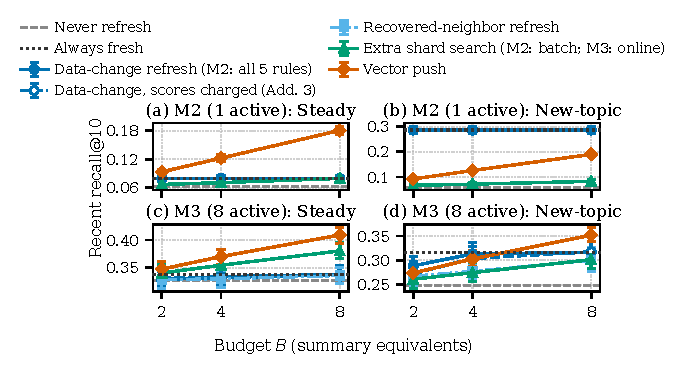
\includegraphics[width=\columnwidth]{figures/fig_m2_m3_budget.pdf}
\caption{Recent recall@10 across $B \in \{2, 4, 8\}$ at $Q{=}200$ in M2 (top, batch ES; all $5$ equal AF) and M3 (bottom, online ESO); y-axes differ. Dashed blue (c, d): data-change with its \RNumDCScoreEpochBytes{} B/epoch of score messages charged ($n_B \in \{1, 3, 7\}$; exploratory Addendum 3, M3 only). Error bars: unpaired per-method \RNumCIPct{} CIs, overlapping even where paired gaps in Table~\ref{tab:m2_m3_equal_bytes} exclude zero (Panel c, $B{=}2$: SS is \RNumMThreeSSMinusDCBTwoSteady{} above plotted DC).}
\label{fig:equal_bytes_b}
\end{figure}

\begin{table}[!t]
\centering
\caption{Refresh Rules and Baselines ($Q{=}200$, Recent Recall@10; St.: steady; NT: new-topic; NR: never refresh; RR: round-robin; DC: data-change; RN: recovered-neighbor; QL: query-popularity; SS: shard-size; AF: always fresh; M2 omitted: all $5$ tie AF; DC is the uncharged rule; charged gaps are in Table~\ref{tab:add3}).}
\label{tab:refresh_rules}
\scriptsize
\renewcommand{\arraystretch}{0.68}
\setlength{\tabcolsep}{1.6pt}
\begin{tabular}{@{}llccccccc@{}}
\toprule
\textbf{Cond.} & \textbf{Str.} & \textbf{NR} & \textbf{RR} & \textbf{DC} & \textbf{RN} & \textbf{QL} & \textbf{SS} & \textbf{AF} \\
\midrule
M1 ($B{=}4$) & St. & \RNumMOneNRRecentSteady{} & \RNumMOneRRRecentSteady{} & \RNumMOneDCRecentSteady{} & \RNumMOneRNRecentSteady{} & \RNumMOneQLRecentSteady{} & \RNumMOneSSRecentSteady{} & \RNumMOneAFRecentSteady{} \\
M3 ($B{=}2$) & St. & \RNumMThreeNRRecentSteady{} & \RNumMThreeRRRecentBTwoSteady{} & \RNumMThreeDCRecentBTwoSteady{} & \RNumMThreeRNRecentBTwoSteady{} & \RNumMThreeQLRecentBTwoSteady{} & \RNumMThreeSSRecentBTwoSteady{} & \RNumMThreeAFRecentSteady{} \\
M3 ($B{=}4$) & St. & \RNumMThreeNRRecentSteady{} & \RNumMThreeRRRecentBFourSteady{} & \RNumMThreeDCRecentBFourSteady{} & \RNumMThreeRNRecentBFourSteady{} & \RNumMThreeQLRecentBFourSteady{} & \RNumMThreeSSRecentBFourSteady{} & \RNumMThreeAFRecentSteady{} \\
M3 ($B{=}8$) & St. & \RNumMThreeNRRecentSteady{} & \RNumMThreeRRRecentBEightSteady{} & \RNumMThreeDCRecentBEightSteady{} & \RNumMThreeRNRecentBEightSteady{} & \RNumMThreeQLRecentBEightSteady{} & \RNumMThreeSSRecentBEightSteady{} & \RNumMThreeAFRecentSteady{} \\
M1 ($B{=}4$) & NT & \RNumMOneNRRecentNewTopic{} & \RNumMOneRRRecentNewTopic{} & \RNumMOneDCRecentNewTopic{} & \RNumMOneRNRecentNewTopic{} & \RNumMOneQLRecentNewTopic{} & \RNumMOneSSRecentNewTopic{} & \RNumMOneAFRecentNewTopic{} \\
M3 ($B{=}2$) & NT & \RNumMThreeNRRecentNewTopic{} & \RNumMThreeRRRecentBTwoNewTopic{} & \RNumMThreeDCRecentBTwoNewTopic{} & \RNumMThreeRNRecentBTwoNewTopic{} & \RNumMThreeQLRecentBTwoNewTopic{} & \RNumMThreeSSRecentBTwoNewTopic{} & \RNumMThreeAFRecentNewTopic{} \\
M3 ($B{=}4$) & NT & \RNumMThreeNRRecentNewTopic{} & \RNumMThreeRRRecentBFourNewTopic{} & \RNumMThreeDCRecentBFourNewTopic{} & \RNumMThreeRNRecentBFourNewTopic{} & \RNumMThreeQLRecentBFourNewTopic{} & \RNumMThreeSSRecentBFourNewTopic{} & \RNumMThreeAFRecentNewTopic{} \\
M3 ($B{=}8$) & NT & \RNumMThreeNRRecentNewTopic{} & \RNumMThreeRRRecentBEightNewTopic{} & \RNumMThreeDCRecentBEightNewTopic{} & \RNumMThreeRNRecentBEightNewTopic{} & \RNumMThreeQLRecentBEightNewTopic{} & \RNumMThreeSSRecentBEightNewTopic{} & \RNumMThreeAFRecentNewTopic{} \\
\bottomrule
\end{tabular}
\end{table}

\begin{table}[!t]
\centering
\caption{Exploratory Addendum 3: Charged Data-Change Minus Each Method (Recent Recall@10 Gaps in pp, \RNumCIPct{} CIs;
charged DC sends $n_B \in \{1, 3, 7\}$ summaries and leaves \RNumAddThreeDCUnspentEpochBytes{} B/epoch of $B$ unspent; X1: vs.\ RN at equal $n_B$; X2: vs.\ PV and ESO; X3: vs.\
uncharged DC; X4: M1, $Q{=}800$, $B{=}4$; ES/ESO: batch/online extra search; PV: vector push;
$^\dagger$fragile, see text).}
\label{tab:add3}
\scriptsize
\renewcommand{\arraystretch}{0.68}
\setlength{\tabcolsep}{3.0pt}
\begin{tabular}{@{}llll@{}}
\toprule
Set ($B$) & Minus & Steady Stream (pp) & New-Topic Stream (pp) \\
\midrule
M3 ($2$) & X1 RN & \RNumAddThreeXOneRNBTwoSteadyCell{} & \RNumAddThreeXOneRNBTwoNewTopicCell{} \\
         & X2 PV & \RNumAddThreeXTwoPVBTwoSteadyCell{} & \RNumAddThreeXTwoPVBTwoNewTopicCell{} \\
         & X2 ESO & \RNumAddThreeXTwoESOBTwoSteadyCell{} & \RNumAddThreeXTwoESOBTwoNewTopicCell{} \\
         & X3 DC & \RNumAddThreeXThreeDCBTwoSteadyCell{} & \RNumAddThreeXThreeDCBTwoNewTopicCell{}$^\dagger$ \\
M3 ($4$) & X1 RN & \RNumAddThreeXOneRNBFourSteadyCell{} & \RNumAddThreeXOneRNBFourNewTopicCell{} \\
         & X2 PV & \RNumAddThreeXTwoPVBFourSteadyCell{} & \RNumAddThreeXTwoPVBFourNewTopicCell{} \\
         & X2 ESO & \RNumAddThreeXTwoESOBFourSteadyCell{} & \RNumAddThreeXTwoESOBFourNewTopicCell{} \\
         & X3 DC & \RNumAddThreeXThreeDCBFourSteadyCell{} & \RNumAddThreeXThreeDCBFourNewTopicCell{} \\
M3 ($8$) & X1 RN & \RNumAddThreeXOneRNBEightSteadyCell{} & \RNumAddThreeXOneRNBEightNewTopicCell{} \\
         & X2 PV & \RNumAddThreeXTwoPVBEightSteadyCell{} & \RNumAddThreeXTwoPVBEightNewTopicCell{} \\
         & X2 ESO & \RNumAddThreeXTwoESOBEightSteadyCell{} & \RNumAddThreeXTwoESOBEightNewTopicCell{}$^\dagger$ \\
         & X3 DC & \RNumAddThreeXThreeDCBEightSteadyCell{} & \RNumAddThreeXThreeDCBEightNewTopicCell{} \\
M1 ($4$) & X4 ES & \RNumAddThreeXFourESSteadyCell{} & \RNumAddThreeXFourESNewTopicCell{}$^\dagger$ \\
         & X4 ESO & \RNumAddThreeXFourESOSteadyCell{} & \RNumAddThreeXFourESONewTopicCell{} \\
         & X4 PV & \RNumAddThreeXFourPVSteadyCell{} & \RNumAddThreeXFourPVNewTopicCell{} \\
         & X4 DC & \RNumAddThreeXFourDCSteadyCell{} & \RNumAddThreeXFourDCNewTopicCell{} \\
\bottomrule
\end{tabular}
\end{table}

\subsection{Arrival-Time Segment Placement (M2 and M3)}
\label{sec:results_m2_m3}

\textbf{Single-segment placement (M2: PR2, GT2, H3, H4).} Epoch $e$ writes only to shard $e \bmod 32$, which every rule refreshes at $B \ge 2$, matching AF in all \RNumMTwoSeedStreamBudgetConds{} conditions (PR2: \RNumPredMTwoTiesGap{}, max diff \RNumPredMTwoTiesMaxAbs{}; Table~\ref{tab:hypotheses}). Re-sending $n_B - 1$ unmodified summaries ($\mu_s^{\text{cand}} = \mu_s^{\text{pub}}$) consumes \RNumMTwoUnmodShareBTwo{}, \RNumMTwoUnmodShareBFour{}, and \RNumMTwoUnmodShareBEight{} of $B$ for the four zero-overhead rules; a deployment could save those bytes or mix in vector push or extra search (not tested). Every pairwise refresh gap in H3 is \RNumHThreeGapZero{} (failing H3 by construction), and the $A = 8$ sensitivity runs (seeds \RNumSeedMin{} to \RNumSensSeedMax{}) match M2 on every query ($3$-seed means \RNumSensRecallMeanSteady{} steady, \RNumSensRecallMeanNewTopic{} new-topic). The value of refreshing that active shard splits by stream (Fig.~\ref{fig:equal_bytes_b}a,b, Table~\ref{tab:m2_m3_equal_bytes}). On steady, \RNumSteadyEpochInsertVecs{} random vectors from all topics land on shard $e \bmod 32$ each epoch, and never-refresh gets \RNumMTwoNRRecentSteady{} recent recall@10, matching $m / S = 2 / 32 = {}$\RNumChanceRecallMTwo{} chance (all-shard \RNumMTwoAllShardsRecentSteady{}; oracle by overall neighbors \RNumMTwoOracleRecentSteady{}). Plausibly because \RNumCentersPerSummary{} centers cannot represent a uniform topic mix, always-fresh reaches only \RNumMTwoAFRecentSteady{} (\RNumGateMTwoSteady{}, failing GT2) and changes overall recall@10 from \RNumMTwoNROverallSteady{} to \RNumMTwoAFOverallSteady{} (\RNumGateMTwoOverallSteady{}, negative in every seed). Vector push therefore wins on steady at every $B$ (H4, Table~\ref{tab:m2_m3_equal_bytes}): pushing \RNumMTwoPVShareBTwo{}, \RNumMTwoPVShareBFour{}, and \RNumMTwoPVShareBEight{} of new vectors at $B \in \{2, 4, 8\}$ gives \RNumMTwoPVRecentBTwoSteady{}, \RNumMTwoPVRecentBFourSteady{}, and \RNumMTwoPVRecentBEightSteady{} ($R_{\text{NR}} + p(1 - R_{\text{NR}}) = {}$\RNumMTwoPVPredRecentBTwoSteady{}, \RNumMTwoPVPredRecentBFourSteady{}, and \RNumMTwoPVPredRecentBEightSteady{}). On new-topic, arrivals come from one or two held-out clusters that \RNumCentersPerSummary{} centers fit cleanly: always-fresh jumps from \RNumMTwoNRRecentNewTopic{} to \RNumMTwoAFRecentNewTopic{} (\RNumGateMTwoNewTopic{}, passing GT2; oracle \RNumMTwoOracleRecentNewTopic{}, all-shard \RNumMTwoAllShardsRecentNewTopic{}) and raises overall recall@10 from \RNumMTwoNROverallNewTopic{} to \RNumMTwoAFOverallNewTopic{} (\RNumGateMTwoOverallNewTopic{}). Across $B \in \{2, 4, 8\}$ on new-topic (H4, Table~\ref{tab:m2_m3_equal_bytes}), fresh summaries beat batch extra search and vector push on recent recall@10, narrowing as $B$ pushes more vectors while \RNumOneSummary{} summary suffices. On overall recall@10, they beat vector push by \RNumHFourRefMinusPVOverallBTwoNewTopic{}, \RNumHFourRefMinusPVOverallBFourNewTopic{}, and \RNumHFourRefMinusPVOverallBEightNewTopic{}.\looseness=-1

\textbf{Eight-segment placement ($G = 8$, M3: GT3, H3b, PR3, H4b) and Exploratory Addendum 3 (X1 to X3).} With $G = 8$ active shards per epoch, steady arrivals mix topics on each active shard: never-refresh is \RNumMThreeNRRecentSteady{} and always-fresh is \RNumMThreeAFRecentSteady{} (oracle \RNumMThreeOracleRecentSteady{}, all-shard \RNumMThreeAllShardsRecentSteady{}). Full refresh fails GT3 on steady (\RNumGateMThreeSteady{}) and changes overall recall@10 by \RNumGateMThreeOverallSteady{} (negative in all five seeds). On new-topic, GT3 passes in aggregate, raising recent recall@10 from \RNumMThreeNRRecentNewTopic{} to \RNumMThreeAFRecentNewTopic{} (\RNumGateMThreeNewTopic{}, overall \RNumGateMThreeOverallNewTopic{}; oracle \RNumMThreeOracleRecentNewTopic{}, all-shard \RNumMThreeAllShardsRecentNewTopic{}), though seed \RNumGateMThreeNewTopicMinSeed{} is \RNumGateMThreeNewTopicMinSeedGap{} ($< {}$\RNumGateThresholdPP{}) and the $t$-interval is \RNumGateMThreeNewTopicTInt{} (unweighted mean \RNumGateMThreeNewTopicUnweightedMean{}). On new-topic at $B = 4$ (Table~\ref{tab:refresh_rules}), H3b fails: recovered-neighbor (\RNumMThreeRNRecentBFourNewTopic{}) loses to data-change (\RNumMThreeDCRecentBFourNewTopic{}) by \RNumHThreeBRNMinusDCNewTopic{} (overall \RNumHThreeBRNMinusDCOverallNewTopic{}, $t$-interval \RNumHThreeBRNMinusDCOverallNewTopicTInt{}). Recovered-neighbor does not differ reliably from query-popularity (\RNumMThreeQLRecentBFourNewTopic{}, \RNumHThreeBRNMinusQLNewTopic{}, positive in all \RNumFiveSeeds{} seeds, $t$-interval \RNumHThreeBMThreeRNMinusQLNewTopicTInt{}) or shard-size (\RNumMThreeSSRecentBFourNewTopic{}, \RNumHThreeBRNMinusSSNewTopic{}), and beats only round-robin (\RNumMThreeRRRecentBFourNewTopic{}, \RNumHThreeBRNMinusRRNewTopic{}). Round-robin's cursor advances $n_B \in \{2, 4\}$ shards/epoch while the active group advances $G{=}8$, often refreshing shards whose new vectors are no longer recent and doing no better than never-refresh (\RNumMThreeRRMinusNRBTwoNewTopic{} at $B{=}2$, \RNumMThreeRRMinusNRBFourNewTopic{} at $B{=}4$). Exploratory Addendum 3 (Table~\ref{tab:add3}) shows that recovered-neighbor loses mainly through shard choice. It charges data-change's \RNumDCScoreEpochBytes{} score B/epoch ($n_B \in \{1, 3, 7\}, A \in \{64, 22, 10\}$, leaving \RNumAddThreeDCUnspentEpochBytes{} B/epoch unspent), so both rules refresh equally often, while RN still spends \RNumAddThreeRNExtraEpochBytesVsChargedDC{} B/epoch more plus its uncharged \RNumRNSetupBroadcastBytes{}-B setup broadcast. At equal $n_B$ on new-topic (X1), charged data-change beats recovered-neighbor at $B = 4$ (P1; $t$-interval \RNumAddThreeXOneRNBFourNewTopicTInt{}; overall \RNumAddThreeXOneRNOverallBFourNewTopic{}, $t$-interval crossing zero) and $B = 8$, with all \RNumAddThreeXOnePosSeedsBFourBEight{} seed gaps positive, but not reliably at $B = 2$ or on steady. By linearity, the \RNumHThreeBRNMinusDCNewTopicAbsMean{} H3b gap at $B{=}4$ splits into \RNumAddThreeXOneRNBFourNewTopicAbsMean{} from shard choice at $n_B{=}3$ (\RNumAddThreeXOneChoiceShareBFour{}) and \RNumAddThreeXThreeDCBFourNewTopicAbsMean{} from the extra summary (at $B{=}2$: \RNumAddThreeRNMinusUnchargedDCBTwoNewTopicAbsMean{} splits into \RNumAddThreeXOneRNBTwoNewTopicAbsMean{} and \RNumAddThreeXThreeDCBTwoNewTopicAbsMean{}, whose $t$-interval crosses zero). That extra summary exists because, in main runs, probing uses \RNumRNOverheadEpochBytes{} B/epoch (\RNumRNOverheadShareBTwo{}, \RNumRNOverheadShareBFour{}, \RNumRNOverheadShareBEight{} of $B \in \{2, 4, 8\}$; modified-only cutoffs would not raise $n_B$), leaving $n_B \in \{1, 3, 7\}$, while data-change's score bytes are uncharged ($n_B \in \{2, 4, 8\}$). At $n_B{=}3$ on new-topic ($B{=}4$), RN had \RNumAddThreeRNForcedSumBFourNewTopic{} cap-forced refreshes across \RNumAddThreeTotalRefreshesBFour{} versus \RNumAddThreeChargedDCForcedSumBFourNewTopic{} for charged DC. In the \RNumSpearmanZeroEpochsNewTopicMThree{}/\RNumEpochsPerCondition{} all-zero probe epochs (ties broken by shard ID), the X1 gap averaged \RNumAddThreeXOneAllZeroGapBFourNewTopic{} (\RNumAddThreeXOneAllZeroQueriesBFourNewTopic{} queries) versus \RNumAddThreeXOneNonZeroGapBFourNewTopic{} across the other \RNumSpearmanPairedNNewTopicMThree{} epochs (\RNumAddThreeXOneNonZeroQueriesBFourNewTopic{} queries). At $B = 8$ (PR3), the four uncharged $n_B = 8$ rules match always-fresh on every query (\RNumPredMThreeBEightFourRulesGap{}, max diff \RNumPredMThreeBEightFourRulesMaxAbs{}), whereas charged data-change ($n_B = 7$) no longer ties always-fresh (X3, Table~\ref{tab:add3}). Recovered-neighbor ($n_B = 7$) differs from always-fresh at $B = 8$ by \RNumPredMThreeBEightRNGapSteady{} on steady and \RNumPredMThreeBEightRNGapNewTopic{} on new-topic (max per-query recall difference \RNumPredMThreeBEightRNMaxAbs{}, that is, \RNumPredMThreeBEightRNMaxAbsPP{}, on single-recent-neighbor queries).\looseness=-1

Across $B \in \{2, 4, 8\}$ in eight-segment placement (H4b, Fig.~\ref{fig:equal_bytes_b}c,d, Table~\ref{tab:m2_m3_equal_bytes}), vector push wins at every $B$ on steady (\RNumMThreePVRecentBTwoSteady{}, \RNumMThreePVRecentBFourSteady{}, and \RNumMThreePVRecentBEightSteady{}, matching $R_{\text{NR}} + p(1 - R_{\text{NR}}) = {}$\RNumMThreePVPredRecentBTwoSteady{}, \RNumMThreePVPredRecentBFourSteady{}, and \RNumMThreePVPredRecentBEightSteady{}). On new-topic, vector push beats never refresh by about \RNumMThreePVNewTopicExcessMin{} to \RNumMThreePVNewTopicExcessMax{} more than uniform sampling predicts, plausibly because it takes the newest tail of each cluster-ordered epoch batch (not tested). On new-topic with score bytes uncharged, data-change (\RNumMThreeDCRecentBTwoNewTopic{}) beats online extra search (\RNumMThreeESORecentBTwoNewTopic{}) and leads vector push (\RNumMThreePVRecentBTwoNewTopic{}, overall \RNumHFourBRefMinusPVOverallBTwoNewTopic{}) at $B = 2$. At $B = 4$, it beats online extra search with no clear winner against vector push (\RNumHFourBRefMinusPVBFourNewTopic{}; overall \RNumHFourBRefMinusPVOverallBFourNewTopic{}). At $B = 8$ on new-topic, refresh leads online extra search by \RNumHFourBRefMinusESOBEightNewTopic{} ($t$-interval \RNumHFourBRefMinusESOBEightNewTopicTInt{} crosses zero) while losing to vector push (\RNumMThreePVRecentBEightNewTopic{}) on both metrics (\RNumHFourBRefMinusPVBEightNewTopic{}; overall \RNumHFourBRefMinusPVOverallBEightNewTopic{}). That overall gain scans $\le {}$\RNumPVMaxVecsBEight{} retained vectors, whereas a $W \cdot N_{\text{push}}$ FIFO buffer suffices for recent recall. The uncharged $B = 2$ lead over vector push (\RNumHFourBRefMinusPVBTwoNewTopic{}) is fragile: its lower CI bound is \RNumHFourBRefMinusPVBTwoNewTopicLow{}, seed \RNumHFourBDCMinusPVBTwoNewTopicNegSeed{} is \RNumHFourBDCMinusPVBTwoNewTopicNegSeedGap{}, and the $t$-interval (\RNumHFourBDCMinusPVBTwoNewTopicTInt{}) crosses zero. In Exploratory Addendum 3 (X2, Table~\ref{tab:add3}), charging data-change's \RNumDCScoreEpochBytes{} score bytes/epoch cuts it from \RNumFourRulesSummariesBTwo{} to \RNumOneSummary{} summary at $B = 2$ and removes that lead. Charged data-change minus vector push is \RNumAddThreeXTwoPVBTwoNewTopic{} (P2; $t$-interval \RNumAddThreeXTwoPVBTwoNewTopicTInt{}), although it is ahead on overall recall@10 (\RNumAddThreeXTwoPVOverallBTwoNewTopic{}). At $B = 4$ there is no clear winner, and vector push leads at $B = 8$ on new-topic and at every $B$ on steady. Against online extra search on new-topic, charged data-change does not lead reliably at $B{=}2$, leads at $B{=}4$, and leads fragilely at $B{=}8$ ($t$-interval \RNumAddThreeXTwoESOBEightNewTopicTInt{}, seed \RNumAddThreeXTwoESOBEightNewTopicNegSeed{} at \RNumAddThreeXTwoESOBEightNewTopicNegSeedGap{}). It trails on overall recall@10 at $B{=}4$ (\RNumAddThreeXTwoESOOverallBFourNewTopic{}; $t$-interval crosses zero) and $B{=}8$ (\RNumAddThreeXTwoESOOverallBEightNewTopic{}). Batch ES adds \RNumESLoadPctBTwo{}, \RNumESLoadPctBFour{}, and \RNumESLoadPctBEight{} extra HNSW load at $B \in \{2, 4, 8\}$. Its LK gaps are \RNumLookaheadMThreeBTwoSteady{}, \RNumLookaheadMThreeBFourSteady{}, and \RNumLookaheadMThreeBEightSteady{} on steady and \RNumLookaheadMThreeBTwoNewTopic{}, \RNumLookaheadMThreeBFourNewTopic{}, and \RNumLookaheadMThreeBEightNewTopic{} on new-topic. ESO spends \RNumMThreeESOShareOfESMin{} to \RNumMThreeESOShareOfESMax{} of ES bytes (\RNumMThreeESOShareOfRefreshBTwoNewTopic{} to \RNumMThreeESOShareOfRefreshBTwoSteady{} of refresh at $B{=}2$). Under the ES slope across budgets, its unspent searches are worth about \RNumMThreeESOUnderspendValMin{} to \RNumMThreeESOUnderspendValMax{}, changing no H4b winner but confounding LK.\looseness=-1

\subsection{Rank Correlation, Starvation Cap, and Threats}
\label{sec:results_diagnostics}

\begin{table}[!t]
\centering
\caption{Mean Spearman $\rho$ with Lift-In Counts and Cap Shares (\RNumEpochsPerCondition{} Epochs/Cond.; St.: steady; NT: new-topic; Def.: defined-$\rho$ epochs, means on Def.; RN-Const.: epochs (\% of \RNumEpochsPerCondition{}) with \RNumSampleQueries{}-query estimate all zero while lift-in counts vary; Cap: $w(s){>}A$ RN share).}
\label{tab:spearman}
\scriptsize
\renewcommand{\arraystretch}{0.68}
\setlength{\tabcolsep}{2.5pt}
\begin{tabular}{@{}llcccc@{}}
\toprule
\textbf{Cond.} & \textbf{Str.} & \textbf{$\rho(\text{RN})$} & \textbf{$\rho(N_{\text{new}})$} & \textbf{Def., RN-Const.\ (\%)} & \textbf{Cap} \\
\midrule
M1 ($Q{=}50$) & St. & \RNumSpearmanRNSteadyMOneQFifty{} & \RNumSpearmanNewVecsSteadyMOneQFifty{} & \RNumSpearmanPairedNSteadyMOneQFifty{}, \RNumSpearmanZeroEpochsSteadyMOneQFifty{} (\RNumSpearmanZeroPctSteadyMOneQFifty{}) & \RNumForcedShareRNSteadyMOneQFifty{} \\
M1 ($Q{=}200$) & St. & \RNumSpearmanRNSteadyMOne{} & \RNumSpearmanNewVecsSteadyMOne{} & \RNumSpearmanPairedNSteadyMOne{}, \RNumSpearmanZeroEpochsSteadyMOne{} (\RNumSpearmanZeroPctSteadyMOne{}) & \RNumForcedShareRNSteadyMOne{} \\
M1 ($Q{=}800$) & St. & \RNumSpearmanRNSteadyMOneQEightHundred{} & \RNumSpearmanNewVecsSteadyMOneQEightHundred{} & \RNumSpearmanPairedNSteadyMOneQEightHundred{}, \RNumSpearmanZeroEpochsSteadyMOneQEightHundred{} (\RNumSpearmanZeroPctSteadyMOneQEightHundred{}) & \RNumForcedShareRNSteadyMOneQEightHundred{} \\
M1 ($Q{=}50$) & NT & \RNumSpearmanRNNewTopicMOneQFifty{} & \RNumSpearmanNewVecsNewTopicMOneQFifty{} & \RNumSpearmanPairedNNewTopicMOneQFifty{}, \RNumSpearmanZeroEpochsNewTopicMOneQFifty{} (\RNumSpearmanZeroPctNewTopicMOneQFifty{}) & \RNumForcedShareRNNewTopicMOneQFifty{} \\
M1 ($Q{=}200$) & NT & \RNumSpearmanRNNewTopicMOne{} & \RNumSpearmanNewVecsNewTopicMOne{} & \RNumSpearmanPairedNNewTopicMOne{}, \RNumSpearmanZeroEpochsNewTopicMOne{} (\RNumSpearmanZeroPctNewTopicMOne{}) & \RNumForcedShareRNNewTopicMOne{} \\
M1 ($Q{=}800$) & NT & \RNumSpearmanRNNewTopicMOneQEightHundred{} & \RNumSpearmanNewVecsNewTopicMOneQEightHundred{} & \RNumSpearmanPairedNNewTopicMOneQEightHundred{}, \RNumSpearmanZeroEpochsNewTopicMOneQEightHundred{} (\RNumSpearmanZeroPctNewTopicMOneQEightHundred{}) & \RNumForcedShareRNNewTopicMOneQEightHundred{} \\
M3 ($B{=}2$) & St. & \RNumSpearmanRNSteadyMThreeBTwo{} & \RNumSpearmanNewVecsSteadyMThreeBTwo{} & \RNumSpearmanPairedNSteadyMThreeBTwo{}, \RNumSpearmanZeroEpochsSteadyMThreeBTwo{} (\RNumSpearmanZeroPctSteadyMThreeBTwo{}) & \RNumForcedShareRNSteadyMThreeBTwo{} \\
M3 ($B{=}4$) & St. & \RNumSpearmanRNSteadyMThree{} & \RNumSpearmanNewVecsSteadyMThree{} & \RNumSpearmanPairedNSteadyMThree{}, \RNumSpearmanZeroEpochsSteadyMThree{} (\RNumSpearmanZeroPctSteadyMThree{}) & \RNumForcedShareRNSteadyMThree{} \\
M3 ($B{=}8$) & St. & \RNumSpearmanRNSteadyMThreeBEight{} & \RNumSpearmanNewVecsSteadyMThreeBEight{} & \RNumSpearmanPairedNSteadyMThreeBEight{}, \RNumSpearmanZeroEpochsSteadyMThreeBEight{} (\RNumSpearmanZeroPctSteadyMThreeBEight{}) & \RNumForcedShareRNSteadyMThreeBEight{} \\
M3 ($B{=}2$) & NT & \RNumSpearmanRNNewTopicMThreeBTwo{} & \RNumSpearmanNewVecsNewTopicMThreeBTwo{} & \RNumSpearmanPairedNNewTopicMThreeBTwo{}, \RNumSpearmanZeroEpochsNewTopicMThreeBTwo{} (\RNumSpearmanZeroPctNewTopicMThreeBTwo{}) & \RNumForcedShareRNNewTopicMThreeBTwo{} \\
M3 ($B{=}4$) & NT & \RNumSpearmanRNNewTopicMThree{} & \RNumSpearmanNewVecsNewTopicMThree{} & \RNumSpearmanPairedNNewTopicMThree{}, \RNumSpearmanZeroEpochsNewTopicMThree{} (\RNumSpearmanZeroPctNewTopicMThree{}) & \RNumForcedShareRNNewTopicMThree{} \\
M3 ($B{=}8$) & NT & \RNumSpearmanRNNewTopicMThreeBEight{} & \RNumSpearmanNewVecsNewTopicMThreeBEight{} & \RNumSpearmanPairedNNewTopicMThreeBEight{}, \RNumSpearmanZeroEpochsNewTopicMThreeBEight{} (\RNumSpearmanZeroPctNewTopicMThreeBEight{}) & \RNumForcedShareRNNewTopicMThreeBEight{} \\
\bottomrule
\end{tabular}
\end{table}

\textbf{Spearman rank correlation and starvation cap.} Table~\ref{tab:spearman} compares mean Spearman $\rho$ across \RNumNumShards{} shards between lift-in counts and $\text{raw}_{\text{rn}}(s)$ vs.\ $N_{\text{new}}(s)$ on RN runs ($\rho$ for DC not measured; $N_{\text{new}}(s)$ not tested as a rule). In M1, RN's refreshes, estimate, and Cap are independent of $Q$ ($Q_s{=}64$), whereas lift-in counts depend on $Q$ and are all zero in \RNumSpearmanZeroTrueSteadyMOneQFifty{} (steady) and \RNumSpearmanZeroTrueNewTopicMOneQFifty{} (new-topic) epochs at $Q{=}50$ and \RNumSpearmanZeroTrueSteadyMThreeBEight{} and \RNumSpearmanZeroTrueNewTopicMThreeBEight{} epochs of M3 $B{=}8$ (outside Def.\ and RN-Const.). In every centroid and eight-segment condition, mean $\rho(\text{RN})$ is below $\rho(N_{\text{new}})$ (means without CIs over epochs where $\text{raw}_{\text{rn}}(s)$ varies, favoring the probe). Counterfactually on data-change runs at $Q{=}200, B{=}4$, $\rho(\text{RN})$ vs.\ $\rho(N_{\text{new}})$ is \RNumSpearmanRNOnDCSteadyMOne{} vs.\ \RNumSpearmanNewVecsOnDCSteadyMOne{} and \RNumSpearmanRNOnDCNewTopicMOne{} vs.\ \RNumSpearmanNewVecsOnDCNewTopicMOne{} in M1, and \RNumSpearmanRNOnDCSteadyMThree{} vs.\ \RNumSpearmanNewVecsOnDCSteadyMThree{} and \RNumSpearmanRNOnDCNewTopicMThree{} vs.\ \RNumSpearmanNewVecsOnDCNewTopicMThree{} in M3. By contrast, $\text{raw}_{\text{rn}}(s) = 0$ across all \RNumNumShards{} shards in every RN-Const.\ epoch of Table~\ref{tab:spearman}, giving zero ranking signal from \RNumRNOverheadEpochBytes{} probe bytes and falling back to $w(s) > A$ and ascending shard ID $s$. In M2, $\rho$ is \RNumSpearmanDegenerateMTwo{} in every defined epoch ($1$ modified shard/epoch). Because $\text{raw}_{\text{ql}}(s)$ and $\text{raw}_{\text{ss}}(s)$ do not reset on refresh, $w(s) > A$ forces \RNumForcedShareQLSteadyMOne{} to \RNumForcedShareSSSteadyMOne{} (steady) and \RNumForcedShareSSNewTopicMOne{} to \RNumForcedShareQLNewTopicMOne{} (new-topic) of QL and SS refreshes at $Q{=}200, B{=}4$ in M1 (vs.\ \RNumForcedShareDCSteadyMOne{} and \RNumForcedShareDCNewTopicMOne{} for DC).\looseness=-1

\textbf{Threats to validity.} First, Section~\ref{sec:system}'s six uncharged costs affect policies differently (RN's \RNumRNSetupBroadcastBytes{}-B setup broadcast and local compute, ES HNSW load, coordinator vector scans, and DC's \RNumDCScoreEpochBytes{} score B/epoch in main runs). Exploratory Addendum 3 charged DC's score bytes ($n_B \in \{1, 3, 7\}$), removing data-change's $B{=}8$ PR3 tie (\RNumAddThreeXThreeDCBEightNewTopic{} vs.\ always-fresh) and $B{=}2$ H4b lead (\RNumAddThreeXTwoPVBTwoNewTopic{} vs.\ vector push) and leaving a fragile $Q{=}800$ recent-recall lead over batch extra search (\RNumAddThreeXFourESNewTopic{}). Even so, charged data-change beat recovered-neighbor at $n_B{=}3$ by \RNumAddThreeXOneRNBFourNewTopic{} on new-topic despite recovered-neighbor spending \RNumAddThreeRNExtraEpochBytesVsChargedDC{} bytes/epoch more plus its uncharged setup broadcast. Because the zero-slack floor leaves \RNumAddThreeDCUnspentEpochBytes{} bytes/epoch unspent for charged data-change (and \RNumRNStrandedEpochBytesBFour{} bytes/epoch for recovered-neighbor at $B{=}4$), this charge is a pessimistic integer-packing case; we did not run a carryover variant, under which \RNumDCScoreEpochBytes{} bytes/epoch totals $< 1$ summary over \RNumNumEpochs{} epochs. Second, in M2 and M3, arrivals append to shards keeping initial topic clusters; on steady, rebuilding \RNumCentersPerSummary{}-center summaries over mixed shards changes overall recall@10 by \RNumGateMTwoOverallSteady{} and \RNumGateMThreeOverallSteady{} (AF minus NR), plausibly shifting centers toward random arrivals (not tested; per-segment summaries not modeled). Both placements also assume a schedule-oblivious coordinator routing only by $\mu_s^{\text{pub}}$; routing directly to known active shards ($e \bmod S$ or the $G$ active shards scored by setup centroids) costs zero maintenance bytes (not tested). Third, at $\approx {}$\RNumSteadyEpochInsertVecs{} inserts/epoch, summary size is fixed while the arrival share buffered by PV (\RNumMTwoPVShareBTwo{}, \RNumMTwoPVShareBFour{}, \RNumMTwoPVShareBEight{} on steady) falls as inserts grow, which may favor refresh at higher ingest rates (not tested). Fourth, all runs use one embedding model (\RNumVectorDimFloats{}-float MiniLM on \RNumCorpusTotalPassages{} MS MARCO passages, data seed \RNumDataSeed{}), fixed $S{=}32, m{=}2, c{=}16$, and $5$ seeds (\RNumSeedMin{} to \RNumSeedMax{}; $3$ in Sens).\looseness=-1

\section{Conclusion}
\label{sec:conclusion}

Where to spend a per-epoch budget $B$ to recover recent top-$10$ neighbors depends on vector placement and topic drift. Under centroid placement, setup summaries already guide queries to shards receiving new vectors, so full refresh every epoch changes recent recall@10 over never refreshing by only \RNumHOneGapSteady{} on steady and \RNumHOneGapNewTopic{} on new-topic. At $Q = 200, B = 4$, causal online extra search and vector push beat every refresh rule on both streams. Data-change refresh overtakes extra search only on new-topic at $Q = 800$, by \RNumQSweepRefMinusESQEightHundredNewTopicAbsMean{} uncharged and \RNumAddThreeXFourESNewTopicAbsMean{} with its score bytes charged (fragile, not ahead on overall recall@10), while trailing vector push. Under arrival-time placement, \RNumCentersPerSummary{}-center summaries fail to summarize random steady arrivals and change overall recall@10 by \RNumGateMTwoOverallSteady{} and \RNumGateMThreeOverallSteady{} when refreshed, leaving vector push ahead at every $B$. On new-topic arrivals, refreshing active summaries raises recent recall@10 by \RNumGateMTwoNewTopic{} in single-segment placement and \RNumGateMThreeNewTopic{} in eight-segment placement, beating vector push across $B \in \{2, 4, 8\}$ in single-segment placement. In eight-segment placement on new-topic, refresh has no clear winner against vector push at $B = 4$ and loses at $B = 8$. At $B = 2$ it edges vector push only with score bytes uncharged; charging them costs a whole summary under the zero-slack floor and leaves no lead (\RNumAddThreeXTwoPVBTwoNewTopic{}). There, at $B = 4$, recovered-neighbor loses to data-change by \RNumHThreeBRNMinusDCNewTopic{} with score bytes uncharged, mainly because the probe picks worse shards. With data-change's \RNumDCScoreEpochBytes{} score bytes/epoch charged so both get \RNumRNSummariesBFour{} refreshes, data-change still leads by \RNumAddThreeXOneRNBFourNewTopic{}; the other \RNumAddThreeXThreeDCBFourNewTopicAbsMean{} comes from the one refresh that probing (\RNumRNOverheadShareBFour{} of $B$) takes away. The probe's estimate correlates less strongly with lift-in neighbor counts than $N_{\text{new}}(s)$ on average in every centroid and eight-segment condition.\looseness=-1

For coordinator-routed vector stores in our tested regime ($S = 32, m = 2, c = 16$, $\approx {}$\RNumSteadyEpochInsertVecs{} inserts/epoch), these results suggest three rules accounting for uncharged costs. (1) Under centroid placement at $Q \le 200$, spend bytes on causal online extra search if shards can absorb up to \RNumExtraSearchesBFour{} more HNSW searches/epoch (\RNumESOQFiftyMaxSearches{} at $Q = 50$) and \RNumThreeShards{}-shard fan-out (or an extra round trip). Alternatively, spend them on vector push if the coordinator can buffer and scan recent vectors (\RNumPVMaxVecsBFour{} vectors at $B = 4$). Reserve summary refresh for higher query rates under topic drift, where data-change refresh overtook extra search at $Q = 800$ (fragilely once its score bytes are charged) but trailed vector push. (2) Under arrival-time placement without schedule-aware routing, refresh the active shard summary when arrivals cluster by topic into one segment. On new-topic with $G = 8$ active segments, fresh summaries and vector push are close at $B \le 4$ and vector push leads at $B = 8$. Avoid rebuilding \RNumCentersPerSummary{}-center $k$-means summaries on shards mixing all topics uniformly; there, vector push recovers recent neighbors while leaving the setup summaries, and so routing, unchanged. (3) When scheduling refreshes across active shards, rank shards by the data-change score rather than paying \RNumRNOverheadEpochBytes{} bytes/epoch (plus setup broadcast) for \RNumSampleQueries{}-query cutoff probing. With its \RNumDCScoreEpochBytes{} bytes/epoch charged, data-change still beat the probe at equal refreshes on new-topic at $B \in \{4, 8\}$. The new-vector count $N_{\text{new}}(s)$ tracked lift-in neighbor counts better than the probe in every centroid and eight-segment condition, though it was not tested as a refresh rule. Because summary size is fixed while PV's buffered arrival share at fixed $B$ falls as inserts grow, higher ingest rates may favor refresh (not tested). Beyond our single-process simulator on \RNumCorpusTotalPassages{} MS MARCO MiniLM vectors, future work should test adaptive summaries, schedule-aware routing, higher ingest rates, and tail latency.\looseness=-1


\section*{Acknowledgment}
Gemini (Google) drafted the simulator, analysis code, figure and number scripts, and the text of every section.
Claude (Anthropic) checked each citation against its source, recomputed reported numbers, and wrote or edited
text in every section. Gemini, Claude, and Codex (OpenAI) reviewed drafts; Codex edited no files. Result numbers
come from scripts run on stored run outputs. \ifanonymous The authors take\else The author takes\fi{} responsibility for the content.

\bibliographystyle{IEEEtran}
\bibliography{bstctl,refs}

\end{document}
